\documentclass[11pt]{article}
\usepackage{palatino}
\usepackage{setspace}
\usepackage{geometry}
\geometry{a4paper, margin=1in}
\usepackage{fancyhdr}
\pagestyle{fancy}\fancyhf{}\renewcommand{\headrulewidth}{0pt}\fancyfoot[C]{\thepage}
\usepackage{amsmath, amssymb, amsfonts}
\usepackage{graphicx}\graphicspath{{../Figures/}}
\usepackage{float}
\usepackage[authoryear]{natbib}
\usepackage{caption}
\usepackage{pdfpages}
\usepackage{booktabs}
\usepackage{url}
\IfFileExists{titlesec.sty}{\usepackage{titlesec}}{}
\IfFileExists{tocloft.sty}{\usepackage{tocloft}}{}
\floatstyle{ruled}
\doublespacing

\begin{document}
\begin{titlepage}
    \centering
    \vspace*{1in}
    {\Large University of Central Florida\par}
    \vspace{0.2in}
    {\large College of Business\par}
    {\large ECO6935–25\par}
    {\large Capstone in Business Analytics I\par}
    \vspace{0.4in}
    {\large Polina Baikova\par}
    \vspace{1in}
    {\LARGE Understanding Housing Market Dynamics and Residential Property Valuation Patterns in Orlando, Florida Using Hedonic Price Modeling\par}
    \vfill
    {\large July 2025\par}
\end{titlepage}
\setcounter{page}{1}
\newpage
\renewcommand{\thesection}{\arabic{section}}
\section*{Introduction and Motivation}

In Florida, housing demand has increased significantly. The Orlando Metropolitan Area has emerged as one of the fastest-growing regions in the United States, leading Florida’s growth statistics in recent years. Forecasts suggest the population may increase by nearly one million by 2045, presenting challenges for housing supply, infrastructure development, and urban planning \citep{bebr:2023}. 

To address these challenges and to inform sound policy and investment decisions, a deeper understanding of the housing market dynamics in Orlando is essential. When exploring housing prices, it is important to account for the full range of characteristics that influence housing prices --- not only physical attributes of a property itself, but neighborhood and locational factors, too.

The Hedonic pricing offers a rigorous, data-driven approach to decompose prices into the implicit values of their underlying characteristics \citep{rosen:1974}. By applying it to real estate and analyzing actual transaction data, this project aims to estimate homebuyers’ valuations of various housing features. The goal is to develop a flexible empirical model that captures how housing attributes influence prices in the Orlando region, offering insight into the structure of demand in this growing urban market and providing a framework that can be extended to other geographic areas.

\section*{Institutional Details}
The residential real estate market in Florida is shaped by a combination of institutional, regulatory, and economic factors that influence both the supply and the demand. The state’s lack of personal income tax and relatively low property taxes have contributed to steady in-migration from other states. Within Florida, the Orlando Metropolitan Area stands out as a key destination due to its economic growth, entertainment infrastructure, and expanding job market.

Orlando’s housing market has undergone substantial transformation over the past decade ($2014$ -- $24$). During this period, the median home price nearly doubled --- from around $\$160,000$ to approximately $\$380,000$ \citep{orra:2024}. Even though part of this growth reflects inflation, a significant portion represents real appreciation driven by sustained demand and population growth. Adjusted for inflation, the 2014 median price would be about $\$257,909$ in $2024$ dollars, indicating notable real gains in property values \citep{bls:2024}.
The Orlando housing market is characterized by a diverse range of property types, from suburban single-family homes to urban condominiums and newly developed subdivisions. 

Local governments, including the county and the city planning boards, regulate land use through zoning ordinances that affect housing density, lot sizes, and permitted property uses. These zoning regulations, along with school district boundaries and proximity to transportation infrastructure, contribute to spatial variations in housing prices across the region.
Home purchases in Florida are typically facilitated through Multiple Listing Services, and prices are determined in a decentralized, market-based system where buyer preferences are revealed through negotiated sales. Property values are also affected by policies such as the Save Our Homes amendment, which limits annual increases in assessed value for owner-occupied homes, and by seasonal factors that drive demand fluctuations throughout the year.

A comprehensive understanding of housing market trends allows homebuyers to make informed purchasing decisions, enables developers to anticipate demand and allocate resources efficiently, assists investors in identifying areas with strong growth potential, and supports policymakers in formulating effective strategies for land use, infrastructure planning, and housing affordability. A rigorous analysis of the factors influencing housing prices is essential for guiding evidence-based decisions in a rapidly evolving urban environment.

\section*{Economic Model}
\subsection*{Hedonic Price Model}
The hedonic price model is built on the notion that the price of a heterogenous good is determined by the combined value of its observed characteristics. This pricing method aims to decompose econometrically the observed variation in the price of a heterogeneous good and isolate the impact of these observed characteristics.

Hedonic pricing model became an established approach in the twentieth century and has generated numerous achievements dealing with theoretical, methodological and empirical research. Kelvin Lancaster’s $1966$ work, ``A New Approach to Consumer Theory" laid the groundwork for the theoretical basis of hedonic modeling. Lancaster argued that utility is not derived from the good as a whole, but from the distinct characteristics it possesses, with total utility reflecting the combined contribution of each individual attribute. Although Lancaster laid the foundation for attribute-based valuation, it was Sherwin Rosen who formally developed the theory of hedonic pricing. In his $1974$ paper, ``Hedonic Prices and Implicit Markets: Product Differentiation in Pure Competition", Rosen argued that a price of a good can be interpreted as the sum of the individual prices of its characteristics. 

Since its introduction, hedonic pricing theory has been widely adopted in housing market research, with many studies exploring how different property and neighborhood features are reflected in market prices through varying methodological approaches.
In the context of housing, each residential unit can be represented by a vector of observable characteristics:
\[
\mathbf z=(z_{1},z_{2},\ldots,z_{k}), \quad \texttt{for} \quad k = 1, 2, ... K
\]
where $z_k$ measures the amount of the $k^{\text{th}}$ attribute that the house contains.
In a competitive housing market, the hedonic price function maps the attribute bundle to its market price:
\[
P(\mathbf z)=f(z_{1},z_{2},\ldots,z_{k})
\]

\subsection*{Consumers side of the market}

\textit{Utility-maximization.}  
Consumer chooses composite consumption $x$ and housing bundle $\mathbf z$ that maximize their utility:  
\[
\max_{x,\mathbf z}\;U(x,\mathbf z)
\quad\text{subject to}\quad
y=x+P(\mathbf z)
\]
\noindent where $y$ denotes income.

\textit{First-order conditions:}  

\[ \frac{\partial U(x,\mathbf z) / \partial z_k}{\partial U (x,\mathbf z)/ \partial x} =  
\frac{\partial p(\mathbf{z})}{\partial z_k} \]

\noindent The right-hand side is the implicit price of attribute $k$; the left-hand side is the marginal rate of substitution between $z_{k}$ and the composite commodity.

\subsection*{Producers side of the market}

Producers supply goods of quality $\mathbf z$ and quantity $q$ to maximize profit:
\[
\max_{q,\mathbf z}\;\pi=qP(\mathbf z)-C(q,\mathbf z)
\]

\noindent Because a single house is typically marketed and sold as an indivisible unit, we will set $q=1$.

\textit{First-order conditions:}
\begin{align*}
\text{(i)} \quad \;&\frac{\partial P(\mathbf z)}{\partial z_{k}}= \frac{\partial C(q,\mathbf z)}{\partial z_{k}}
\\[4pt]
\text{(ii)} \quad \;&P(\mathbf z)=\frac{\partial C(q,\mathbf z)}{\partial q}
\end{align*}
Condition (i) equates the implicit price of improving quality $z_{k}$ to its marginal cost; condition (ii) requires unit price to equal marginal production cost.

\subsection*{Hedonic Equilibrium}

An equilibrium, a house $\mathbf z^{*}$ is traded at a price $P(\mathbf z^{*})$, and there exist a consumer and a producer such that:

\[
\frac{\partial U(x^{*},\mathbf z^{*})/\partial z_{i}}{\partial U(x^{*},\mathbf z^{*})/\partial x}
=
\frac{\partial P(\mathbf z^*)}{\partial z_{k}}
=
\frac{\partial C(q^{*},\mathbf z^{*})}{\partial z_{k}}
\]

\noindent These conditions ensure that: (1) consumers choose $\mathbf z^{*}$ where their marginal willingness to pay equals the implicit price;
(2) producers supply $\mathbf z^{*}$ where their marginal cost equals that same implicit price; and (3) the set of $P(\mathbf z^*)$ pairs satisfying these equalities traces the hedonic price function --- the locus where consumers' bid and producers' offer curves are tangent and the market clears.

Estimation of implicit prices that reveal the consumers' marginal willingness to pay has been the focus of the majority of empirical hedonic analyses and is referred to as the first stage of the hedonic. The second stage involves recovering demand and supply functions for attributes.

This project focuses on the first stage of the hedonic analysis, concentrating on estimating and interpreting the implicit prices from observed housing market transactions.

\section*{Statistical Model }
Hedonic regression is a specialized application of linear regression in which the price of a differentiated good is decomposed into the effect of various attributes. Although the underlying estimation method remains the method of least squares, the key distinction lies in the interpretation: each coefficient in a hedonic model represents the implicit price of a specific characteristic holding all else constant. 

\subsection*{Log-linear Hedonic Regression}
Linear regression is well-suited for this framework because it allows one to estimate how marginal changes in features affect market value. However, since housing attributes often exhibit non-constant effects (particularly diminishing marginal returns) a log-linear specification is typically preferred \citep{abelson:1979}. The log-linear hedonic model takes the following form: 

\[
\log P_n = \beta_0 + \mathbf{w}_n \boldsymbol\gamma + \mathbf{z}_n \boldsymbol\delta + U_n
\]

\noindent where  \( \log P_n \) is a natural logarithm of the sale price for property \(n\), \( \beta_0 \) is an intercept term, \( \mathbf{w}_n \) is a vector of structural characteristics, \( \boldsymbol\gamma \) is a vector of coefficients for structural characteristics, \( \mathbf{z}_n \) is a vector of neighborhood characteristics, \( \boldsymbol\delta \) is a vector of coefficients for neighborhood characteristics, \( U_n \) is an error term capturing unobserved influences for property \(n\).


\subsection*{LASSO Regularization}

Although the log-linear hedonic specification effectively captures the marginal contributions of housing attributes, models with a large number of correlated predictors risk overfitting, which can destabilize coefficient estimates and impair interpretability. Least Absolute Shrinkage and Selection Operator (LASSO) regularization technique can be employed to improve model's generalizability and addresses multicollinearity by prioritizing variables that contribute most to explaining variation in dependent variable.

LASSO augments the standard sum-of-squares objective function with an additional penalty term that imposes an \( \ell_1 \)-norm constraint on the regression coefficients. The optimization problem is defined by the following:

\[
L(\hat{\boldsymbol{\beta}}) = \arg\min_{\boldsymbol\beta}\; \sum_{n=1}^{N} \left( \log P_n - \beta_0 - \mathbf{x}_n^s \boldsymbol \beta \right)^2 + \mu \left\| \boldsymbol\beta_{-1} \right\|_1 
\]

\noindent where \( \log P_n \) is the observed outcome for observation $n$, \( \mathbf{x}_n^s \) denotes the vector of standardized predictors for observation $n$, \( \boldsymbol{\beta} \) represents the vector of coefficients, and \( \mu  \) is a tuning parameter that controls the degree of penalization. Here, $\beta_{-1}$ denotes the vector $\beta$ without the constant $\beta_0$, and the penalty term \( \| \boldsymbol\beta_{-1} \|_1 \) shrinks some coefficients toward zero, thereby performing implicit variable selection. 

\subsection*{Linear Generalized Additive Model}

Although linear regression assumes constant marginal effects for each covariate, the generalized additive model (GAM) relaxes this assumption by allowing the effect of selected continuous variables to vary smoothly over their range. This approach preserves interpretability for linear terms while enabling the model to uncover nonlinear patterns in the data that a single index f the feature variables may fail to detect. 

\[
\log P_n = \beta_0 + \sum_{j} \beta_j x_{nj} + \sum_{k} f_k(z_{nk}) + U_n
\]

\noindent where  \( \ln p_n \) is a natural logarithm of the sale price for property \(n\), \( \beta_0 \) is an intercept term, \( x_{nj} \) are covariates with linear effects for observation \( n \), \( \beta_j \) are the coefficients corresponding to the linear covariates, \( f_k(\cdot) \) are smooth functions represented by penalized splines, estimated for continuous covariates \( z_{nk} \), and \( U_n \) is an error term capturing unobserved influences.

\section*{Empirical Specification}

In this section, I discuss the empirical framework used to estimate the implicit prices of housing attributes through a hedonic price model. I begin by describing the source and structure of the data, followed by the construction of a representative set of structural and neighborhood characteristics relevant to the valuation of residential properties. Next, I outline the rationale for geographically stratifying the analysis to account for spatial heterogeneity in housing markets. Finally, I review the core assumptions of the method of least squares and explain how model coefficients are interpreted within the log-linear specification.

\subsection*{Data Source and Structure}

The empirical analysis is based on a dataset of publicly available records from the Zillow website, focusing on residential properties marked as sold between January $2023$ and May $2025$.

The geographic scope of the study is limited to ZIP codes within the Orlando postal region, defined specifically as areas where the city name is listed as Orlando, FL. This definition ensures consistency in geographic coverage while capturing the urban and suburban variation within Orlando's housing market.

Extensive data cleaning and transformation procedures were conducted using Python. This process involved removing incomplete entries, standardizing formats, and engineering new variables relevant to housing structure, amenities, and location. The final dataset includes complete records on property sale price, sale date, structural features, and locational attributes, along with precise geographic identifiers such as city, county, street address, ZIP code, longitude, latitude. A detailed description of all variables, including their definitions and construction methods, is provided in the Appendix A.

\subsubsection*{Dependent Variable}

The dependent variable is the sale price of each residential property, recorded as the actual transaction price at the time of sale. This measure is of central importance in hedonic analysis, as it captures the revealed preferences of market participants. The observed sale price reflects the marginal willingness to pay for the full bundle of housing attributes associated with each property. Applying the natural logarithm of sale price during modeling is a practical transformation that helps address skewness and stabilize variance, improving the model’s interpretability and performance.

To ensure comparability over time, all prices were adjusted for inflation using the Consumer Price Index for All Urban Consumers \citep{bls:2024}. Prices were converted to constant May 2025 dollars using the formula:

\[
\text{Adjusted Price}_n = \frac{\text{Nominal Price}_i}{\text{CPI}_{t(n)} / \text{CPI}_{\text{May 2025}}}
\]

\noindent where $\text{CPI}_{t(n)}$ is the CPI for the month of sale of property $n$, and
$\text{CPI}_{\text{May 2025}}$ is the CPI for the base period.


\begin{figure}[H]
	\centering
	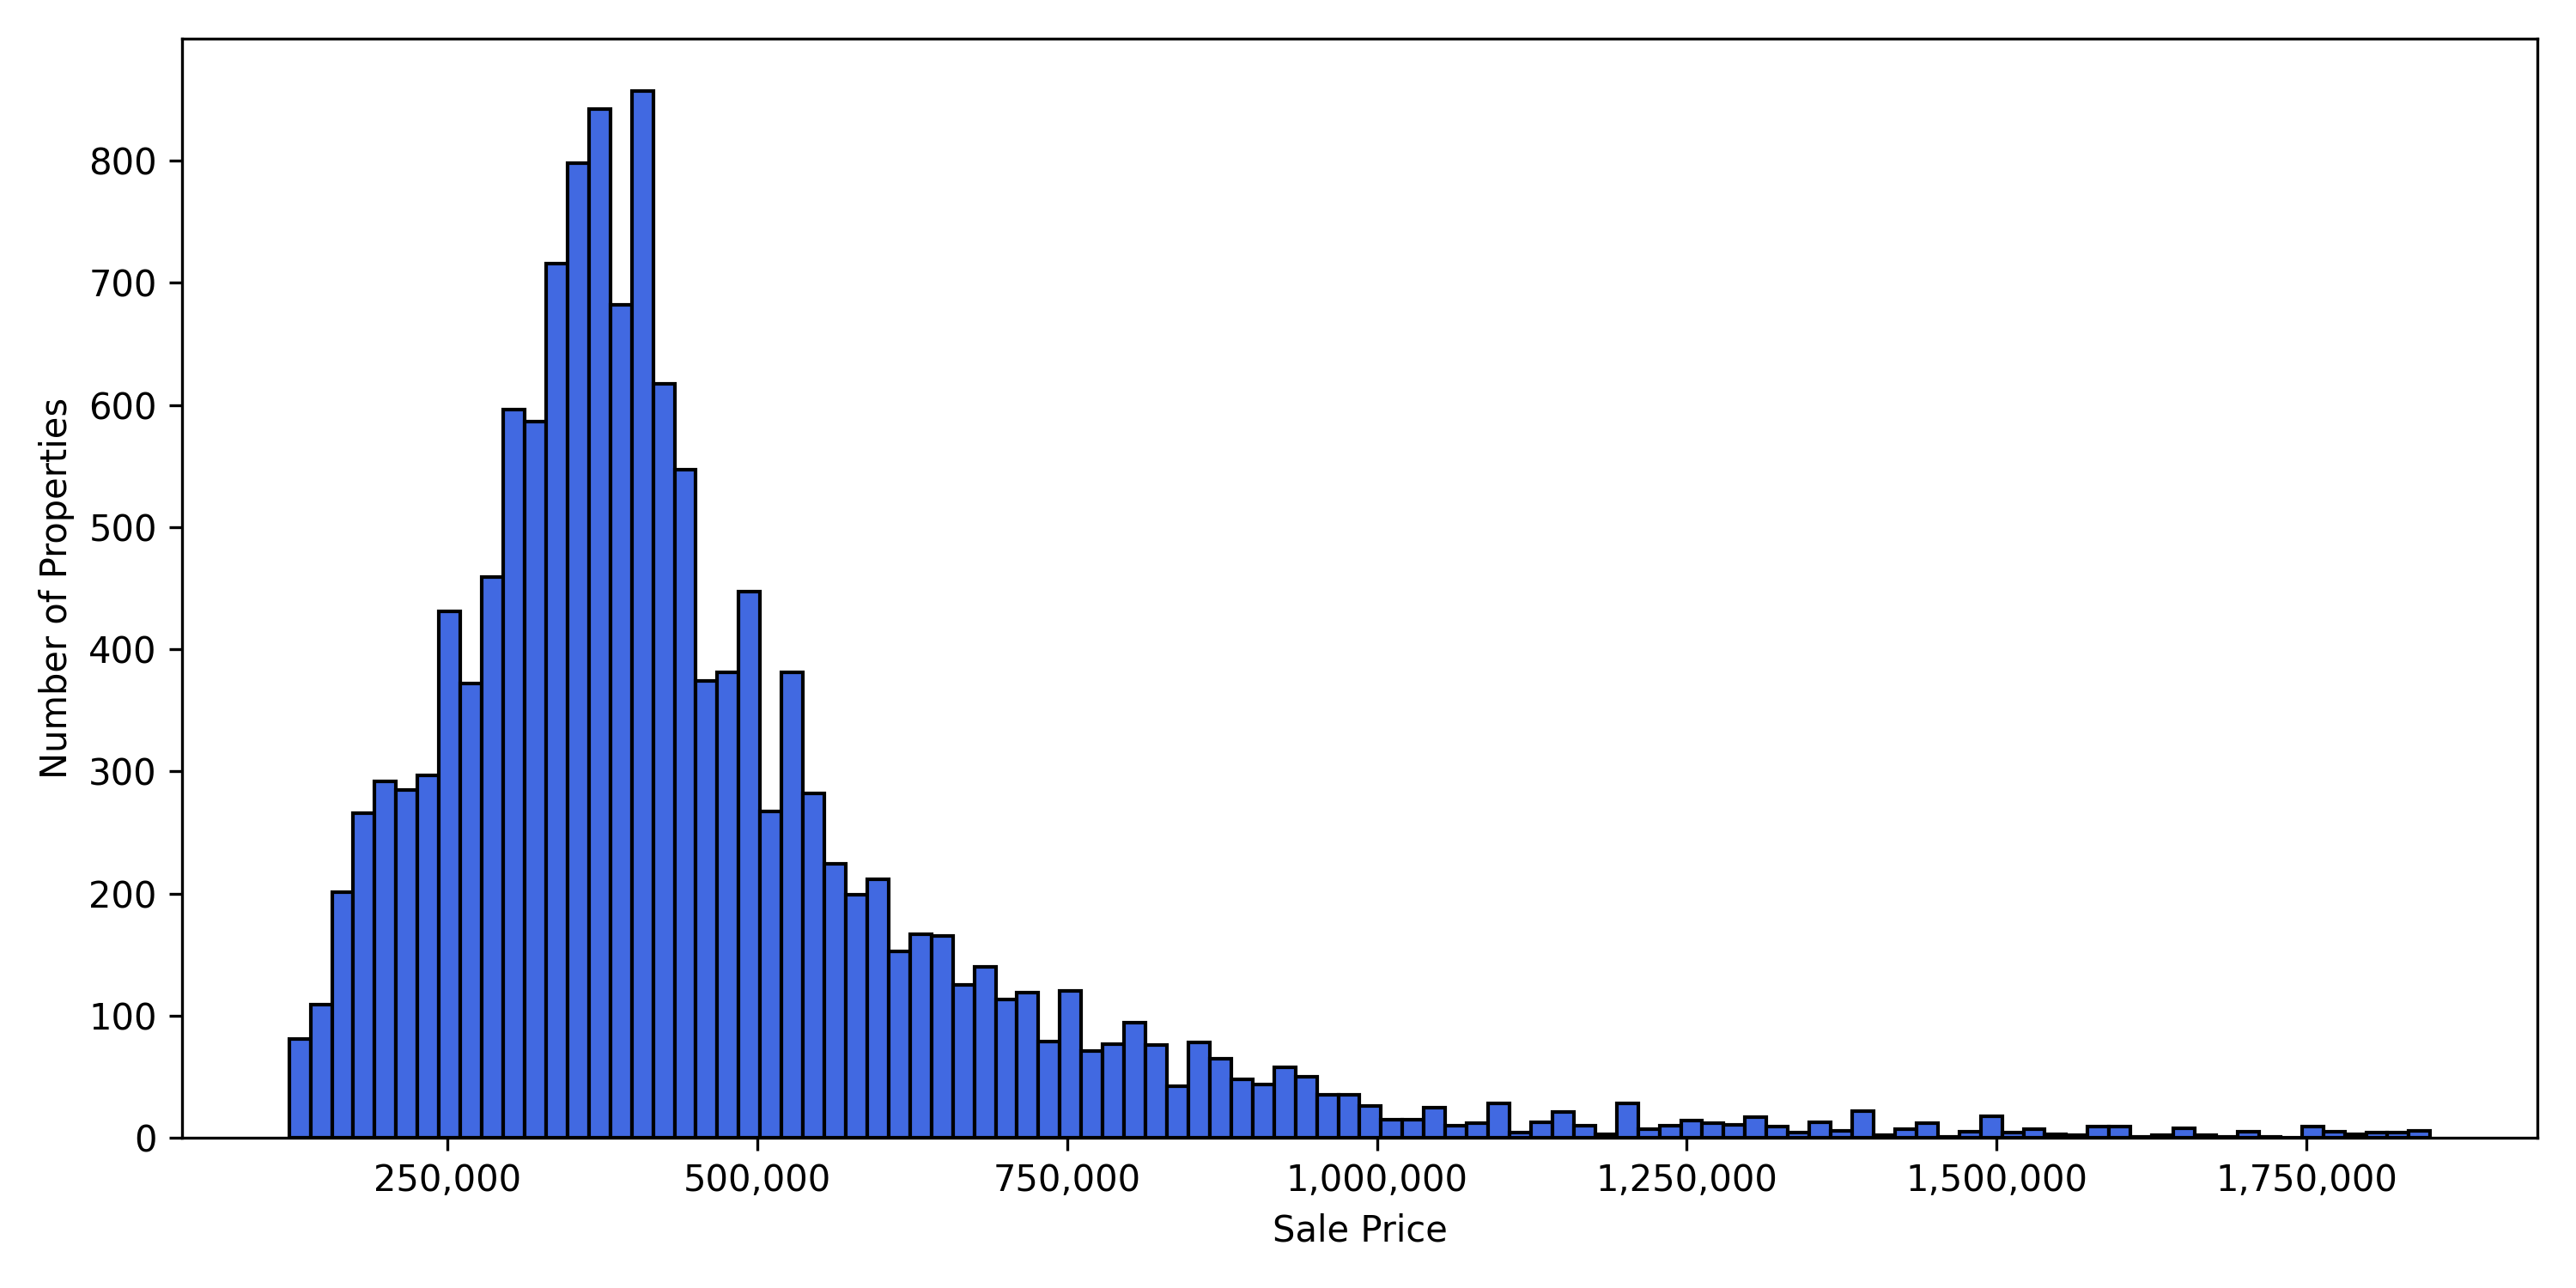
\includegraphics[width=0.9\textwidth]{Figures/sale_price_distribution.png}
    \caption{Distribution of Real Sale Prices in Orlando}
	\label{fig:1}
\end{figure}


\subsubsection*{Structural Characteristics}

Structural characteristics refer to the physical and functional features of each residential property. Variables capturing these characteristics include the type of home, the age of the property (measured as the difference between the sale date and the year built), total living area in square feet, the number of bedrooms and bathrooms, and the number of parking spaces. In addition, binary variables are used to capture the presence of a private pool and a garage.

\subsubsection*{Neighborhood Characteristics}

Neighborhood characteristics capture the broader context in which a property is located and play a key role in shaping buyer preferences beyond structural features. These include binary indicators for the presence of a homeowners’ association (HOA), gated community access, public parks, playgrounds, scenic views, and water views. Recreational amenities are summarized as a count of commonly listed features such as fitness centers, community pools, clubhouses, saunas, spas, and sports courts. Additional variables indicate whether a property is situated outside flood-risk zones, within the official boundaries of the City of Orlando, or adjacent to greenbelt areas comprising natural or agricultural land surrounding urban development. The dataset also includes school-related variables capturing the distance to the nearest elementary, middle, and high schools, as well as their respective ratings based on the GreatSchools rating system.

To assess the effect of proximity to transportation infrastructure on home prices, Manhattan distances were calculated from each property to the nearest exit along I -- $4$, SR -- $408$, SR -- $417$, SR -- $528$, and Florida’s Turnpike. Using \texttt{OpenStreetMap} data retrieved via the \texttt{OSMnx} library, a drivable road network was constructed and filtered to include only major highways and junctions. A custom \texttt{Python} function matched each home to the closest relevant exit based on keyword-matched road names and projected coordinates, producing distance measures in miles (see Appendix B). To simplify the model and to avoid redundancy, only the minimum distance to any of the five highways was retained as the final proximity measure.

\begin{table}
\caption{Summary Statistics}
\label{tab:summary_stats}
\begin{tabular}{lrrrrr}
\toprule
 & mean & std & min & 50\% & max \\
\midrule
sale\_price & 469521.62 & 238104.81 & 123640.77 & 412540.16 & 1976832.37 \\
home\_type & 2.62 & 0.71 & 1.00 & 3.00 & 3.00 \\
age & 29.99 & 20.08 & 1.00 & 29.00 & 108.00 \\
living\_area & 1867.30 & 745.55 & 576.00 & 1682.00 & 5989.00 \\
bedrooms & 3.34 & 0.84 & 1.00 & 3.00 & 8.00 \\
bathrooms & 2.57 & 0.78 & 2.00 & 2.00 & 7.00 \\
avg\_distance\_to\_schools & 1.74 & 0.72 & 0.33 & 1.67 & 5.97 \\
avg\_schools\_rating & 5.21 & 1.43 & 2.67 & 5.00 & 8.33 \\
min\_distance\_highway & 1.73 & 1.18 & 0.04 & 1.48 & 9.27 \\
sqft\_per\_bedroom & 555.20 & 138.73 & 212.00 & 536.00 & 1610.67 \\
\bottomrule
\end{tabular}
\end{table}


\subsection*{Geographic Stratification and Modeling Considerations}

Housing markets are inherently heterogeneous, with both property prices and the implicit prices of individual attributes varying substantially not only between cities, but also across neighborhoods within the same metropolitan area. These variations reflect differences in local market conditions and supply constraints. Even within a single city such as Orlando, housing is not traded in a perfectly competitive market, and preferences can vary widely across subpopulations. From an econometric standpoint, this presents a significant challenge: many utility-relevant characteristics are either unobserved or difficult to quantify, introducing the risk of omitted variable bias and reducing the precision of estimated coefficients \citep{abelson:1979}.

Although the inclusion of a broad set of characteristics generally improves the explanatory power of predictive models, it also introduces practical econometric challenges. By focusing on smaller, more uniform geographic areas, the variability in certain attributes is naturally reduced, which helps address the problem of unobserved heterogeneity and allows for a more parsimonious model specification, thereby improving the stability and interpretability of the estimates.

Therefore, ZIP code data were consolidated into five distinct subregions of Orlando: Orlando Central, Orlando West, Orlando East, Orlando Southeast, and Orlando South. These subregions were defined based on the City of Orlando Commission District boundaries, which reflect administratively relevant, demographically cohesive, and geographically contiguous units. \citep{orangecounty2025}.



\subsection*{Interpretation of Coefficients}

Given the log-linear price function, the marginal implicit price for any individual attribute $z_{nk}$ is given by:

\[
\frac{\partial P_n}{\partial z_{nk}} = \beta_k \, P_n
\]

\noindent This expression indicates that the marginal contribution of a one-unit increase in attribute $z_{nk}$ is proportional to both the estimated coefficient $\beta_k$ and the property's price $P_n$. Because the dependent variable is in logarithmic form, the coefficient $\beta_k$ can be interpreted as the approximate proportional effect on price --- so that $\beta_k \cdot 100$ percent  is the percentage change in price resulting from a one-unit increase in $z_{nk}$, holding all other attributes constant.

\section*{Empirical Results}

\subsection*{Modeling Procedure and Implementation}
The empirical implementation relies on a custom-built \texttt{Python} function designed to estimate log-linear hedonic regression models with enhanced robustness and flexibility. The function integrates tools from \texttt{statsmodels} and \texttt{scikit-learn} to streamline the modeling pipeline. In addition to the linear specification, a separate function was developed to estimate GAM, allowing for nonlinear relationships between selected predictors and the logarithm of sale price. The GAM function utilizes the \texttt{pyGAM} library and incorporates cross-validation for hyperparameter tuning, enabling flexible smoothing of continuous variables while retaining linear treatment of categorical features. Below the results of both the linear and additive hedonic pricing models for residential properties are presented, describing how each was built and refined.


\subsubsection*{Geographic Units of Analysis: Central and East Orlando}
To examine potential spatial heterogeneity in housing attribute valuation, the hedonic model was estimated separately for two Orlando areas. Central Orlando includes ZIP codes $32801$, $32804$, $32806$, $32807$, $32809$, $32812$, $32822$, and $32839$. These ZIP codes correspond to neighborhoods largely within the administrative boundaries of the City of Orlando, including prominent areas such as Downtown Orlando, College Park, Edgewood, Lake Eola Heights, Park Central, and Azalea Park. The area is characterized by a heterogeneous housing stock, including a significant share of older homes constructed in the mid-20th century. This region exhibits median home prices ranging approximately from $\$260,000$ to $\$570,000$, reflecting a broad spectrum of property types, from standard newly constructed houses to historic residences in established neighborhoods such as Lake Como, Colonialtown, and Downtown Orlando. The average population density in this region is approximately 4890 people per square mile, indicating relatively high levels of urbanization.

East Orlando includes ZIP codes $32817$, $32820$, $32826$, and $32828$. This area lies outside the official city limits and represent a more suburban landscape, with extensive residential development occurring primarily from the 1980s onward. It is characterized by large, planned communities such as Avalon Park and Waterford Lakes, along with neighborhoods like Union Park, Alafaya, and the area surrounding the University of Central Florida. The housing stock is more homogeneous, with many properties located within planned subdivisions and exhibiting modern construction standards and layouts. Median home prices in this area range between $\$370,000$ and $\$480,000$, suggesting a relatively narrower distribution compared to Central Orlando. With an average population density of 2440 people per square mile, the region features lower development intensity and greater separation between residential and commercial zones.

Estimating the hedonic model separately across these two regions facilitates comparison of buyer's valuations of structural and neighborhood attributes under distinct urban development contexts.

\subsubsection*{Regularization-Based Feature Selection with LASSO}

To enhance the model's applicability across diverse geographical regions, feature selection is dynamically performed using LASSO regularization. Due to heterogeneity across different housing markets, it is expected that varying attributes will predominantly drive housing prices in different locations. LASSO regression addresses this by penalizing coefficients towards zero, selectively retaining only the most impactful features that significantly contribute to housing prices. 


Following feature selection, the retained subset of variables can be expressed as:
\[
\widehat{S} = \left\{ j \in \{1, \dots, J\} \; : \; \hat{\beta}^{\text{LASSO}}_j \neq 0 \right\}
\]
\noindent where $\widehat{S}$ is the set of indices for predictors retained by the LASSO model. 

\begin{table}
\caption{LASSO Feature Selection Results by Region}
\label{tab:lasso_selection_results}
\begin{tabular}{lll}
\toprule
Feature & Selected: Orlando Central & Selected: Orlando East \\
\midrule
Home Type & Home Type & Home Type \\
Age of Property & Age of Property & Age of Property \\
Bedrooms & Bedrooms & Bedrooms \\
Bathrooms & Bathrooms & Bathrooms \\
Sq. Feet per Bedroom & Sq. Feet per Bedroom & Sq. Feet per Bedroom \\
Number of Stories &  & Number of Stories \\
Number of Parking Spaces &  &  \\
Garage & Garage & Garage \\
Private Pool & Private Pool & Private Pool \\
HOA & HOA & HOA \\
Gated Community & Gated Community & Gated Community \\
Recreational Facilities &  &  \\
Nearby Park & Nearby Park &  \\
Playground Nearby & Playground Nearby & Playground Nearby \\
Greenbelt &  &  \\
Above Flood Plain & Above Flood Plain & Above Flood Plain \\
City Lot & City Lot &  \\
Historic District &  &  \\
Water View & Water View & Water View \\
Average Distance to Schools &  &  \\
Average School Rating & Average School Rating & Average School Rating \\
Min. Distance to Highway & Min. Distance to Highway & Min. Distance to Highway \\
\bottomrule
\end{tabular}
\end{table}



Although LASSO is effective for variable selection, it introduces bias by shrinking coefficients and places the estimated parameter vector on the boundary of the parameter space. As a result, it violates regularity conditions required for standard asymptotic inference, making $t$-statistics, $p$-values, and confidence intervals from the LASSO estimates unreliable \citep{lockhartEtAl:2014}. To enable valid statistical inference, the final step involves re-estimating the least squares model using only the subset of predictors selected by LASSO. This methodology helps in dynamically adapting the model to regional variations while maintaining a robust and interpretable structure.



\subsection*{Model Performance of Least Squares}

\subsubsection*{Model Fit}
The log-linear regression models for Central Orlando and East Orlando demonstrate strong overall fit and predictive accuracy, with $R^2$ values of $0.839$ and $0.920$, respectively. The Root Mean Squared Error (RMSE) is $0.194$ for Central Orlando and $0.087$ for East Orlando, reflecting the average squared prediction error in logarithm of sale prices. These results suggest that a substantial portion of the variation in logarithm of sale prices is explained by the selected housing and neighborhood attributes. Given that the models did not incorporates granular interior features or detailed exterior characteristics, these results reflect a high degree of explanatory power. The overall F-statistics confirm that the models are jointly significant.


\begin{table}[H]
\centering
\caption{Least-Squares Model Fit Statistics: Central Orlando and East Orlando}
\label{tab:model_comparison}
\begin{tabular}{lcc}
\toprule
& \textbf{Orlando Central} & \textbf{Orlando East} \\
\midrule
R-squared           & 0.839  & 0.920 \\
F-statistic                    & 675.9  & 649.3 \\
p-value (F-statistic)          & 0.000  & 0.000 \\
RMSE  & 0.194 & 0.087 \\
\bottomrule
\end{tabular}
\end{table}

\subsubsection*{Residual Diagnostics}

The normality assumption in linear regression requires that the error terms are normally distributed with mean zero and constant variance:

\[
U_n \sim \mathcal{N}(0, \sigma^2)
\]

\noindent This assumption underpins the validity of statistical inference in the method of least squares regression, including confidence intervals and hypothesis tests.


\begin{figure}[H]
	\centering
	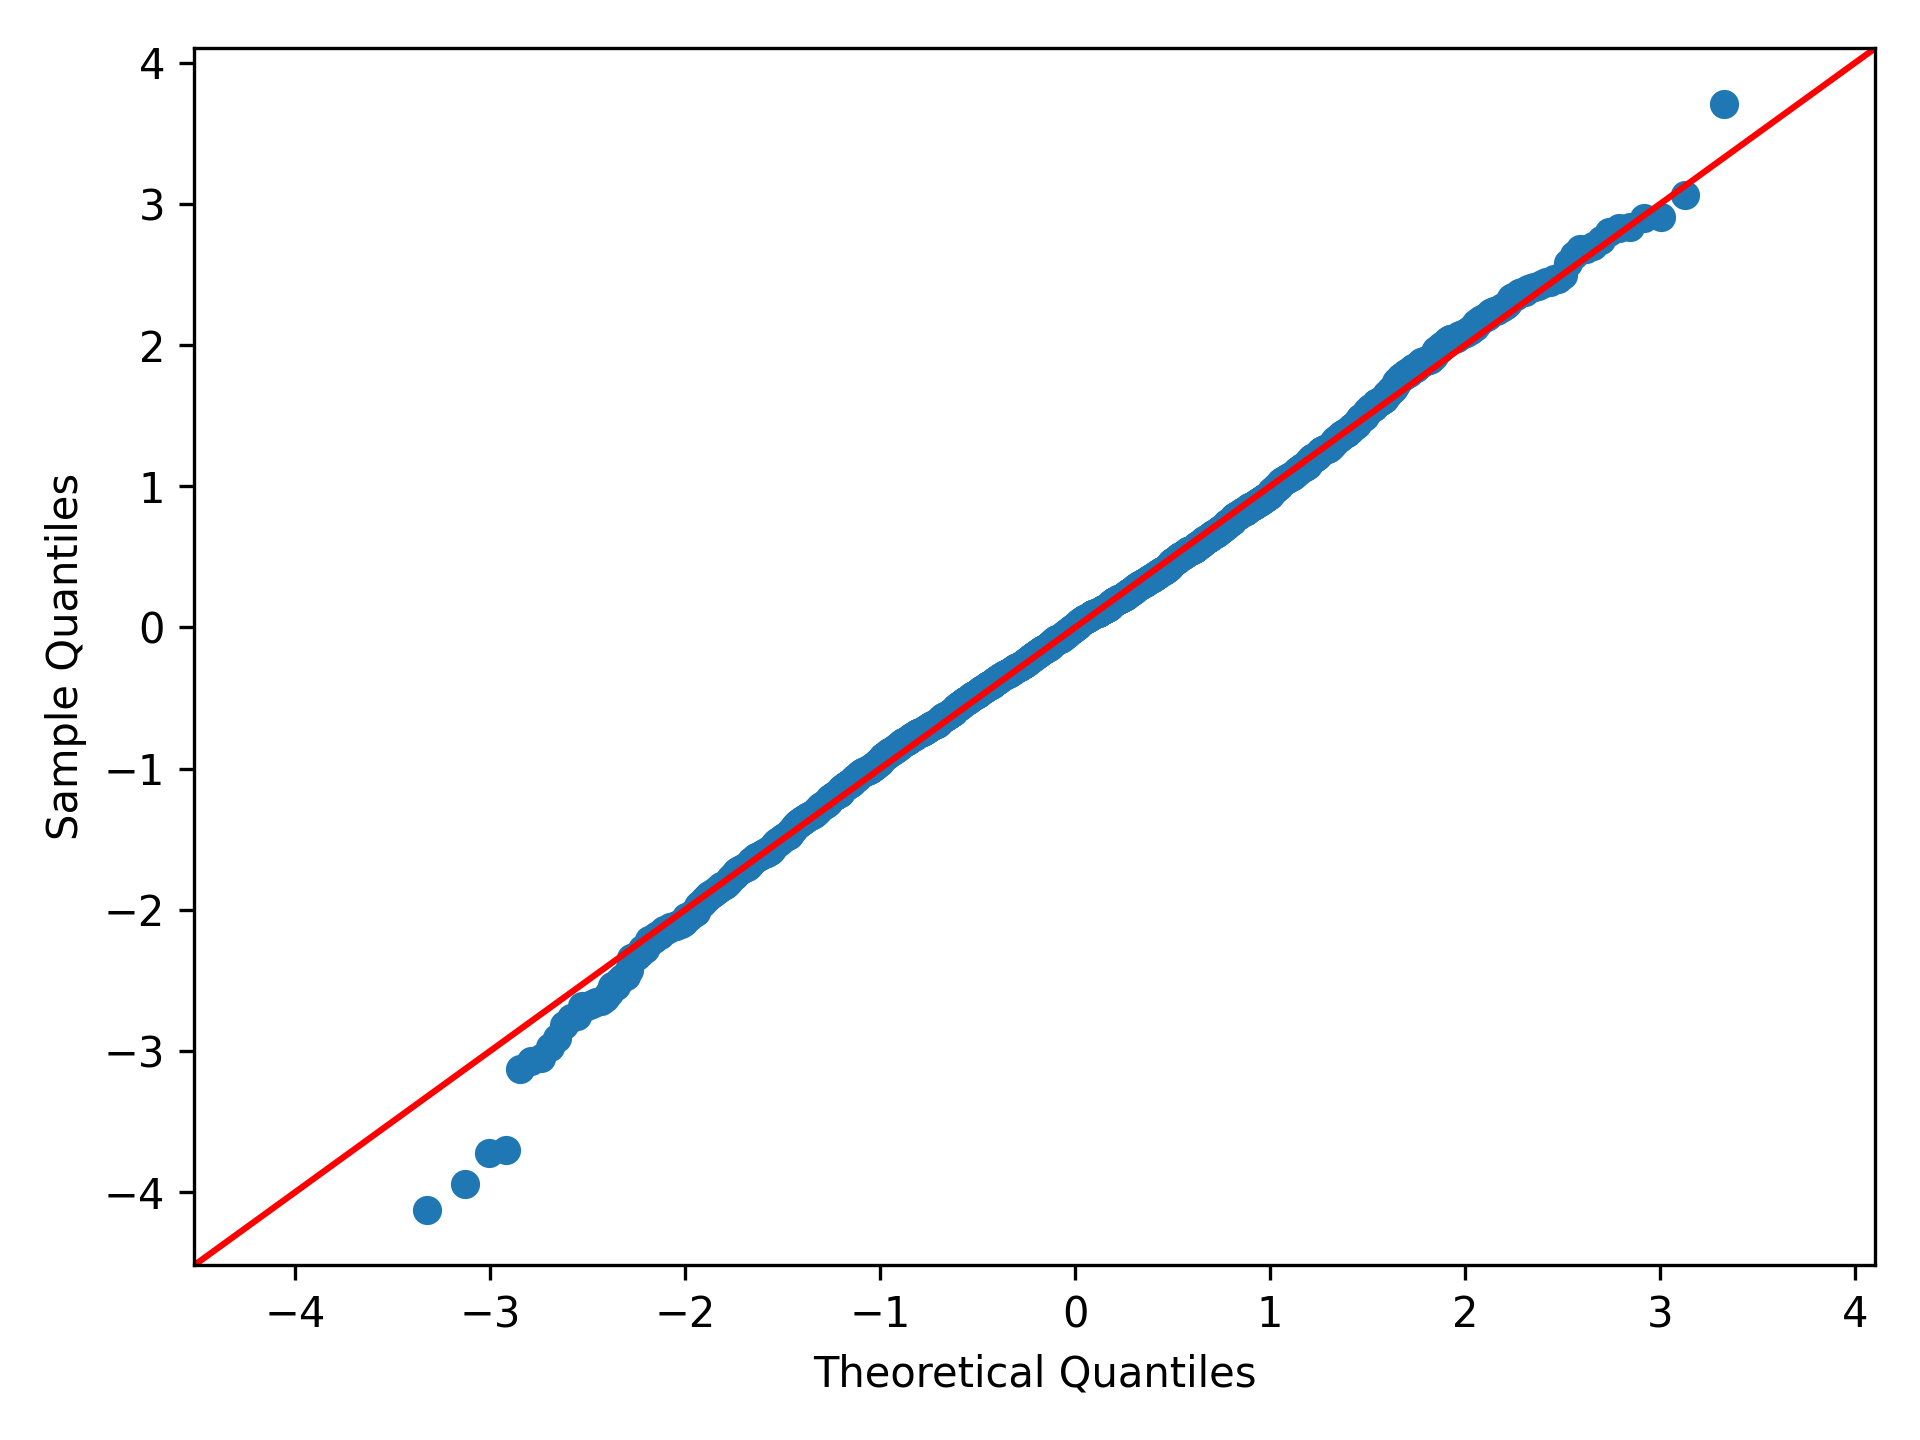
\includegraphics[width=0.7\textwidth]{Figures/qqplot_orlando_central.png}
    \caption{Plot of Residuals for Central Orlando}
	\label{fig:2}
\end{figure}

\begin{figure}[H]
	\centering
	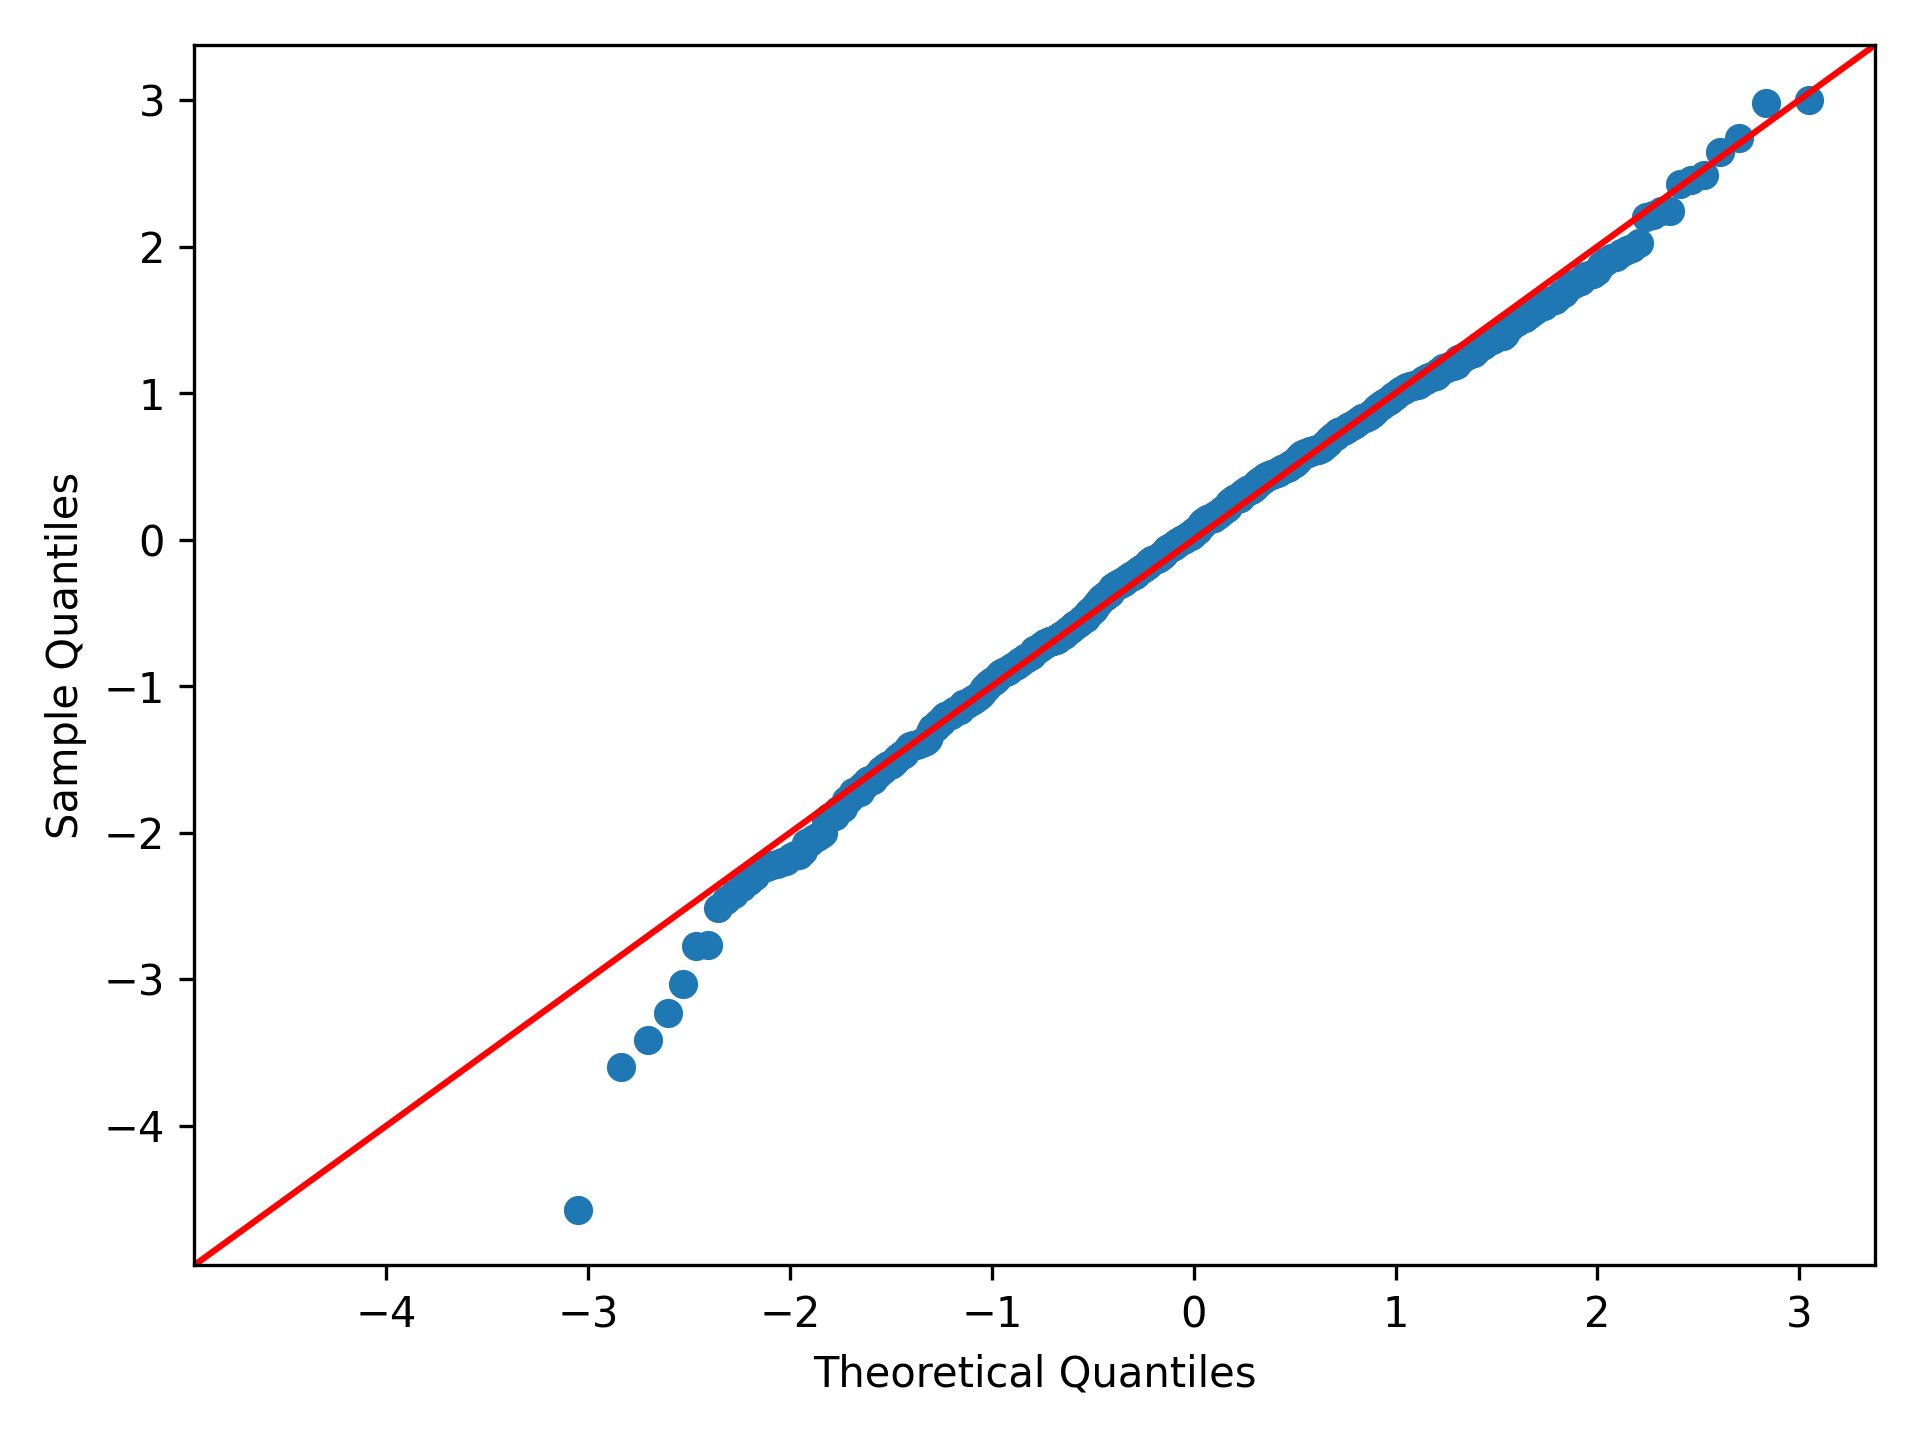
\includegraphics[width=0.7\textwidth]{Figures/qqplot_orlando_east.png}
    \caption{Plot of Residuals for East Orlando}
	\label{fig:3}
\end{figure}


To evaluate whether the residuals satisfy the normality assumption, a Q–Q (quantile–quantile) plot is used to visually compare the empirical distribution of residuals to a theoretical normal distribution. As shown in Figure~\ref{fig:2} and Figure~\ref{fig:3}, the residuals generally align with the 45-degree reference line, with only some deviations in the tails. This suggests that the residuals are approximately normally distributed, supporting the validity of least squares regression inference procedures.

\subsubsection*{Parameter Estimates}


\begin{table}
\caption{Least‑Squares Estimates with 95 percent CI (Central Orlando)}
\label{tab:ols_coeffs_c}
\begin{tabular}{lrrrr}
\toprule
 & Coefficient & Std. Error & CI Lower & CI Upper \\
\midrule
const & 7.4615 & 0.1436 & 7.1800 & 7.7430 \\
Sq. Feet per Bedroom & 0.6664 & 0.0231 & 0.6211 & 0.7117 \\
Home Type & 0.1856 & 0.0085 & 0.1690 & 0.2023 \\
Bedrooms & 0.1851 & 0.0085 & 0.1685 & 0.2017 \\
City Lot & 0.1249 & 0.0136 & 0.0983 & 0.1516 \\
Garage & 0.1089 & 0.0109 & 0.0875 & 0.1302 \\
Above Flood Plain & 0.0850 & 0.0223 & 0.0413 & 0.1287 \\
Bathrooms & 0.0837 & 0.0096 & 0.0649 & 0.1026 \\
Private Pool & 0.0724 & 0.0116 & 0.0496 & 0.0952 \\
Nearby Park & 0.0629 & 0.0150 & 0.0335 & 0.0922 \\
Water View & 0.0512 & 0.0148 & 0.0222 & 0.0802 \\
Average School Rating & 0.0312 & 0.0055 & 0.0205 & 0.0419 \\
Playground Nearby & 0.0254 & 0.0117 & 0.0025 & 0.0483 \\
Gated Community & -0.0165 & 0.0122 & -0.0403 & 0.0074 \\
Age of Property & -0.0224 & 0.0030 & -0.0283 & -0.0166 \\
Min. Distance to Highway & -0.0335 & 0.0054 & -0.0440 & -0.0230 \\
HOA & -0.0997 & 0.0105 & -0.1203 & -0.0792 \\
\bottomrule
\end{tabular}
\end{table}

\begin{table}
\caption{Least‑Squares Estimates with 95 percent CI (East Orlando)}
\label{tab:ols_coeffs_e}
\begin{tabular}{lrrrr}
\toprule
 & Coefficient & Std. Error & CI Lower & CI Upper \\
\midrule
const & 9.3649 & 0.1032 & 9.1626 & 9.5672 \\
Sq. Feet per Bedroom & 0.4329 & 0.0169 & 0.3997 & 0.4661 \\
Home Type & 0.1380 & 0.0108 & 0.1168 & 0.1592 \\
Bedrooms & 0.1238 & 0.0055 & 0.1131 & 0.1345 \\
Private Pool & 0.1188 & 0.0081 & 0.1028 & 0.1347 \\
Above Flood Plain & 0.0811 & 0.0180 & 0.0458 & 0.1165 \\
Garage & 0.0744 & 0.0122 & 0.0505 & 0.0983 \\
Bathrooms & 0.0528 & 0.0076 & 0.0380 & 0.0677 \\
Gated Community & 0.0508 & 0.0110 & 0.0293 & 0.0723 \\
Water View & 0.0379 & 0.0095 & 0.0193 & 0.0565 \\
Average School Rating & 0.0237 & 0.0040 & 0.0159 & 0.0316 \\
Min. Distance to Highway & 0.0145 & 0.0021 & 0.0104 & 0.0185 \\
Playground Nearby & 0.0117 & 0.0073 & -0.0026 & 0.0261 \\
Age of Property & -0.0340 & 0.0027 & -0.0393 & -0.0286 \\
HOA & -0.0526 & 0.0075 & -0.0673 & -0.0379 \\
Number of Stories & -0.0810 & 0.0088 & -0.0982 & -0.0638 \\
\bottomrule
\end{tabular}
\end{table}


The majority of individual coefficients are statistically significant at the $5$ percent level, as shown in Table~~\ref{tab:ols_coeffs_c} and Table~~\ref{tab:ols_coeffs_e}, indicating that their estimated effects on the expected logarithm of sale price are unlikely to be the result of random variation under the null hypothesis of no association.  Reported standard errors are heteroskedasticity-consistent, improving inference in the presence of non-constant error variance. The associated confidence intervals are reasonably narrow, suggesting that the coefficient estimates are stable and estimated with precision.

\subsection*{GAM Model Performance}

\subsubsection*{Model Fit}
To capture potential nonlinearities and diminishing marginal effects common in the housing market, the analysis is extended by using GAM. Housing markets often exhibit complex, non-monotonic relationships, making GAM an appropriate tool for uncovering these patterns. Unlike least squares, which imposes a strictly linear structure, the GAM flexibly models continuous predictors using cubic smoothing splines, allowing the shape of each effect to be determined empirically from the data. Model selection was performed via repeated five-fold cross-validation across a grid of smoothing penalties, with the optimal model chosen to maximize out-of-sample $R^2$. This procedure helps prevent overfitting while ensuring adequate model flexibility. As shown in Table~\ref{tab:model_comparison_gam}, GAM yields a slight improvement in model fit over least squares for both Central and East Orlando, suggesting that allowing for nonlinear effects leads to gains in explanatory power.

\begin{table}[H]
\centering
\caption{GAM Model Fit Statistics:  Central Orlando and East Orlando}
\label{tab:model_comparison_gam}
\begin{tabular}{lcc}
\toprule
 & \textbf{Orlando Central} & \textbf{Orlando East} \\
\midrule
R-squared           & 0.854  & 0.923 \\
RMSE  & 0.178 & 0.080 \\
\bottomrule
\end{tabular}
\end{table}

\subsubsection*{Estimated Effects of Model Predictors}

To interpret the influence of each continuous predictor, finite-difference derivatives of the predicted logarithm of price are computed at the $10^{\text{th}}$, $25^{\text{th}}$, $50^{\text{th}}$, $75^{\text{th}}$, and $90^{\text{th}}$ percentiles of the covariate distribution for each continuous variable. By examining multiple points along the distribution, the analysis captures how price sensitivity to each feature varies with its magnitude. Coefficients for binary variables are interpreted as average log-price differences associated with each respective feature.


As shown in Table \ref{tab:binary_coef_side_by_side}, the GAM‑estimated coefficients for the binary indicators are largely consistent with those obtained from the least squares regression specification, underscoring the robustness of the discrete‑feature effects across the two modeling approaches.

\begin{table}[htbp]
\centering
\caption{GAM Binary Coefficients: Orlando Central and Orlando East}
\label{tab:binary_coef_side_by_side}
\begin{minipage}[t]{0.48\textwidth}
\centering
\caption*{Orlando Central}
\begin{table}[H]
\centering
\begin{tabular}{lr}
\toprule
 & Coefficients \\
\midrule
Home Type & 0.1492 \\
Garage & 0.1180 \\
Private Pool & 0.1023 \\
HOA & -0.0646 \\
Nearby Park & 0.0174 \\
Above Flood Plain & 0.0462 \\
City Lot & 0.0757 \\
Playground Nearby & 0.0261 \\
Water View & 0.0368 \\
\bottomrule
\end{tabular}
\end{table}

\end{minipage}%
\hfill
\begin{minipage}[t]{0.48\textwidth}
\centering
\caption*{Orlando East}
\begin{table}[H]
\centering
\begin{tabular}{lr}
\toprule
 & Coefficients \\
\midrule
Home Type & 0.1307 \\
Garage & 0.0886 \\
Private Pool & 0.1056 \\
HOA & -0.0249 \\
Number of Stories & -0.0724 \\
Gated Community & 0.0437 \\
Above Flood Plain & 0.0325 \\
Playground Nearby & 0.0126 \\
Water View & 0.0336 \\
\bottomrule
\end{tabular}
\end{table}

\end{minipage}
\end{table}

Although GAM binary coefficients confirm discrete-feature effects, examining the derivative-based marginal effects of continuous predictors provides deeper insight into how the influence of these variables varies across the distribution of housing characteristics. As shown in Tables~\ref{tab:orlando_central_marginal} and~\ref{tab:orlando_east_marginal}, these effects are not constant --- some features exhibit diminishing returns or nonlinear patterns, highlighting the value of the GAM framework for uncovering nuanced relationships in the housing market.

Corresponding summary statistics for the percentile values used in the marginal effect analysis, along with plots of the estimated smooth functions for each continuous variable, are provided in the Appendix D.

\begin{table}[H]
\centering
\begin{tabular}{lrrrrr}
\toprule
 & 10\% & 25\% & 50\% & 75\% & 90\% \\
\midrule
Age of Property & -0.1638 & -0.0791 & -0.0167 & 0.0727 & 0.1166 \\
Bedrooms & 0.2320 & 0.2320 & 0.1461 & 0.1461 & 0.1076 \\
Bathrooms & -0.0473 & -0.0473 & -0.0473 & 0.0611 & 0.0611 \\
Sq. Feet per Bedroom & 0.1840 & 0.1782 & 0.1709 & 0.1621 & 0.1525 \\
Average School Rating & 0.0884 & 0.0527 & 0.0238 & 0.0018 & -0.0214 \\
Min. Distance to Highway & 0.0041 & -0.0128 & -0.0246 & -0.0244 & -0.0140 \\
\bottomrule
\end{tabular}
\caption{Orlando Central – Marginal Effects}
\label{tab:orlando_central_marginal}
\end{table}


\begin{table}[H]
\centering
\begin{tabular}{lrrrrr}
\toprule
 & 10\% & 25\% & 50\% & 75\% & 90\% \\
\midrule
Age of Property & -0.1458 & -0.0473 & -0.0109 & 0.0087 & 0.0066 \\
Bedrooms & 0.1138 & 0.1138 & 0.1138 & 0.0934 & 0.0934 \\
Bathrooms & 0.0801 & 0.0801 & 0.0801 & 0.0226 & 0.0226 \\
Sq. Feet per Bedroom & 0.1149 & 0.1075 & 0.1016 & 0.0947 & 0.0891 \\
Average School Rating & 0.0160 & 0.0151 & 0.0138 & 0.0130 & 0.0128 \\
Min. Distance to Highway & -0.0066 & -0.0001 & 0.0120 & 0.0314 & 0.0407 \\
\bottomrule
\end{tabular}
\caption{Orlando East – Marginal Effects}
\label{tab:orlando_east_marginal}
\end{table}



\subsection*{Interpretation Of Results}

The hedonic regression models for Central and East Orlando reveal fundamental housing attributes consistently driving prices, while also highlighting regional differences in attribute valuation. This section examines key findings for each category of variables, emphasizing both universal determinants of value and notable distinctions between urban and suburban contexts.

\textit{Size and Layout.}
Across Central and East Orlando, core structural characteristics significantly impact housing prices. Each additional bedroom increases prices by 18.2 percent  in Central and 12.6 percent in East Orlando, while an additional bathroom adds 7.9 percent and 5.8 percent, respectively. A 10 percent  increase in interior square footage relative to the number of bedrooms results in a 6.6 percent  price premium in Central Orlando and a 4.4 percent premium in East Orlando, reflecting buyers’ preference for more spacious and open layouts. Notably, these features exhibit diminishing marginal returns in the GAM analysis, with marginal effects declining at higher percentiles. Detached single-family homes are valued at approximately 19 percent higher in Central Orlando and 15 percent  higher in East Orlando compared to attached homes. Collectively, these findings suggest greater marginal valuation of space in denser urban markets like Central Orlando, where larger homes and land availability are scarce.

\textit{Property Enhancements.}
Private swimming pools consistently yield positive price premiums, adding approximately 7.7 percent in Central and 11.7 percent  in East Orlando and reflecting strong buyer preferences for comfort and leisure amenities. Garages also add significant value, increasing home prices by 10.9 percent in Central and 8 percent in East Orlando, highlighting demand for secure parking and storage, particularly where urban parking constraints exist. These amenities underscore consistent buyer willingness to pay for features enhancing comfort and convenience.

\textit{School Quality.}
Several neighborhood and environmental factors also demonstrate a consistent influence on prices. School quality, measured by the average rating of nearby schools, positively affects home prices by approximately 3.5 percent  per rating point increase in Central and 2 percent in East Orlando, reinforcing the importance of education access in residential decisions and showing that families with children are willing to bid up home values for access to top-performing schools. The GAM results reveal that this effect is nonlinear in Central Orlando, with stronger marginal gains at lower school quality levels and tapering off at higher ratings, suggesting that buyers place a premium on moving from low- to mid-performing school zones, but the marginal value of additional quality diminishes beyond a certain point. In East Orlando, the effect remains relatively flat across the distribution.

\textit{Floodplain Status.}
Homes situated outside a FEMA-designated high-risk flood zones command price premiums of approximately 7.3 percent in Central and 6.8 percent in East Orlando, reflecting buyer preferences for properties with reduced environmental risks due to concerns about potential damage and the additional cost of insurance. 

\textit{Age.}
The linear regression results indicate that, on average, home values depreciate by approximately 2 percent  per year of age. However, the GAM model reveals that depreciation is not constant, newer homes tend to lose value more quickly, while the marginal effect of age flattens and eventually turns positive for very old homes, particularly in Central Orlando. This pattern is driven by a small number of outliers: older homes in well-established, historically desirable neighborhoods that retain or even gain value over time. Central Orlando, which contains a greater share of such properties, reflects this nonlinearity more clearly. This phenomenon can be understood through the lens of survivorship bias, an economic concept referring to the mistaken inference drawn from observing only entities that have persisted over time, while ignoring those that failed to survive \citep{brownEtAl:1992}. In this context, older homes that remain on the market today tend to be valued as those that were well-built or uniquely located, which skews the observed relationship by making older properties appear more valuable on average.  In contrast, East Orlando shows a flatter relationship between age and price, consistent with its newer housing stock and the near absence of legacy properties.

\textit{Transportation Infrastructure.}
Distinct regional differences further highlight variations in local market dynamics. Proximity to highways demonstrates contrasting effects: In Central Orlando, closer proximity increases home values by about 3.4 percent per mile, reflecting the premium placed on commuting convenience in congested urban areas. In East Orlando, where access is generally easier and neighborhoods are more dispersed, homes farther from highways are valued higher by approximately 1.7 percent per mile, as buyers prioritize tranquility over immediate highway accessibility. The GAM results reinforce these patterns: Central Orlando shows a consistently negative marginal effect, while East Orlando exhibits a nonlinear relationship with positive effects at higher percentiles, suggesting that distance adds value in higher-end segments of the suburban market.

\textit{HOA.}
The presence of homeowners associations negatively influences property values, with a notably stronger impact in Central Orlando, where HOA properties sell for approximately 9.1 percent  less than comparable non-HOA homes. In East Orlando, the effect is smaller, with a price reduction of about 3.5 percent. This difference may reflect varying buyer preferences across urban and suburban contexts; for instance, suburban homeowners might place greater value on amenities and services offered by HOAs. Nevertheless, the consistently negative coefficients suggest that the perceived costs and restrictions associated with HOAs are capitalized into lower sale prices, as buyers adjust their willingness to pay to account for future dues and potential limitations on property use.

\textit{Gated Communities.}
Gated community status has a significant positive effect on home values in East Orlando, where it is associated with a price premium of approximately 6.8 percent. This finding highlights suburban buyers' preferences for security and exclusivity. In contrast, the effect is statistically insignificant in Central Orlando, likely reflecting the scarcity of such developments in dense urban areas. 

\textit{Parks and Green Spaces.}
Public parks and playgrounds proximity significantly benefits Central Orlando properties, increasing values by about 5.9 percent, underscoring the high value urban residents place on accessible recreational green spaces due to limited private outdoor areas. In East Orlando, park proximity is insignificant, given larger private lots and lower population density.

\textit{Views.}
Water views enhance home values consistently, with a 4.8 percent premium in Central and 3.8 percent in East Orlando, reflecting universally positive aesthetic preferences.

\textit{Story Count.}
An interesting result in East Orlando is the negative valuation of multi-story homes, with prices decreasing by approximately 7 percent per additional story. Though seemingly counterintuitive, this aligns with well-established buyer preferences in Florida, particularly among retirees and families with young children, who favor single-level homes for accessibility and ease of maintenance. The state’s warm climate also makes upper floors harder to cool, further reducing their appeal. Appraisers have noted that in some Florida markets, buyers may pay as much for a smaller one-story home as for a larger two-story alternative. The lack of significance for this variable in Central Orlando suggests that this preference is stronger in suburban contexts.

Overall, the side-by-side comparison of Central and East Orlando reveals that the same attributes can carry different weights in different submarkets. These differences highlight the importance of market segmentation in hedonic analysis, while a single unified model for all of Orlando might have missed these nuances. 

\subsubsection*{Connections to Prior Empirical Research}
The observed relationships align with broader real estate research. For example, DiPasquale and Wheaton \citep{dipawill:1996} demonstrated higher marginal values for additional bedrooms in dense urban markets, consistent with findings in Central Orlando. Similarly, the positive premiums for private swimming pools and garages align with research by Sirmans, Macpherson, and Zietz \citep{sirmansEtAl:2006}, who document 5–10 percent  value increases for pools in warm climates and 6–12 percent  for garages.

School quality’s impact echoes findings by Black \citep{black:1999}, illustrating significant price premiums associated with superior schools. Moreover, the observed price discounts for homes in flood-prone areas align with Bin and Polasky \citep{binpola:2004}, who found similar effects in their analysis of environmental risk capitalization.

Regarding HOA effects, Robertson \citep{robertson:2019} and Meltzer and Cheung \citep{meltcheu:2014} both highlighted the negative effects of HOA fees and restrictive covenants on home values, resonating with the negative coefficients observed in Orlando.

Gated community premiums align with the findings of Bible and Hsieh \citep{biblhsie:2001}, indicating small but consistent price increases associated with such neighborhoods in suburban areas.

The impacts of highway proximity observed correspond to findings by Boarnet and Chalermpong \citep{boarchal:2001}, documenting contrasting location preferences in urban versus suburban contexts.

Finally, the negative valuation of multi-story homes aligns with findings by the National Association of Realtors \citep{nar:2020}, noting buyer preferences for single-level homes in retirement-friendly states like Florida.


\section*{Practical Recommendations}

The results of this analysis have practical implications for various stakeholders in the real estate market:

\begin{quote} 

\noindent \textbf{Home buyers:}

\noindent \textit{Make Informed Investment Decisions.} Buyers can use the estimated price effects to spot investment opportunities. A home with features such as a pool, garage, or high school ratings listed below expected value may signal underpricing. In Central Orlando, prioritize space-efficient interiors and parking access; in East Orlando, prioritize homes that offer privacy, recreational amenities, and a quieter residential setting.

\noindent \textit{Avoid Overpaying for Low-Value Attributes.}
\noindent Certain features carry negative or negligible value. Multi-story layouts in East Orlando are associated with lower prices, while HOA restrictions reduce value in both regions. Buyers should factor these effects into their offer and weigh the long-term costs against listed price.

\noindent \textit{Consider Long-Term Resale Potential.}
\noindent Even if certain features, such as proximity to a park, are not a personal priority, their influence on future resale value should not be overlooked.  Homes that score well on high-value attributes tend to maintain or increase value more reliably. 


\noindent \textbf{Sellers:}

\noindent \textit{Highlight High-Value Features.}
In marketing and showings, emphasize attributes that command strong premiums. In Central Orlando, focus on interior space, number of bedrooms and bathrooms, and garage access. In East Orlando, spotlight features like private pools, gated entry, and single-story layout.

\noindent \textit{Make Targeted, Cost-Effective Improvements.}
Renovate selectively. In Central Orlando, consider interior upgrades and additional space. In East Orlando, enhancing outdoor areas or ensuring ease of access for older buyers may yield stronger returns. 

\noindent \textit{Offset Negative Factors.}
If a property lacks key value drivers, it is important to emphasize compensating strengths or propose thoughtful alternatives. For instance, in the absence of a garage, highlighting off-street parking availability can address buyer concerns. Similarly, if proximity to parks or scenic views is limited, showcasing private outdoor areas, quality landscaping, or access to nearby recreational amenities can help convey comparable lifestyle advantages.

\noindent \textbf{Real Estate Developers and Investors:}

\noindent \textit{Incorporate Desirable Site Characteristics.}
Enhance project value by leveraging environmental and locational attributes. In urban developments, proximity to parks and green spaces increases buyer appeal. In flood-prone areas, implement mitigation strategies such as elevated construction and modern drainage to reduce risk. Ensure access to highways or transit, but buffer residential units from traffic-related noise and congestion.

\noindent \textit{Use Data-Driven Strategies.}
Apply hedonic pricing insights to optimize development plans and capital allocation. In compact markets, maximize usable square footage per lot; in suburban settings, offer larger parcels with community features like security gates, walking trails, or shared recreational areas. Grounding design choices in local pricing patterns ensures higher return on investment and market alignment.



\noindent \textbf{City Planners and Policy Makers:}

\noindent \textit{Invest in Public Amenities that Raise Property Values.}
Expanding access to green space in urban areas and improving school outcomes raises surrounding property values. Since property taxes are often based on assessed value, investments in amenities such as parks can directly increase municipal revenue by lifting local home prices.

\noindent \textit{Support Resilient Infrastructure and Risk-Responsive Zoning.}
\noindent Promote land use and infrastructure policies that reflect market preferences and mitigate environmental risks. Invest in drainage systems and flood protection to safeguard property values in vulnerable areas. Encourage zoning flexibility and incentivize development in urban cores to make efficient use of limited land.

\noindent \textit{Improve Urban Transportation and Access.}
\noindent Expand pedestrian, bicycle, and transit infrastructure in city centers to reduce reliance on cars and improve accessibility. Providing convenient access to schools, parks, and commercial services helps sustain long-term property demand.

\end{quote}

\section*{Limitations and Considerations}

Although the hedonic pricing model developed in this study offers meaningful insights into the valuation of housing attributes, several methodological limitations should be acknowledged. These limitations help frame the interpretation of results and point to directions for future research.

As is typical in housing market analyses, it is challenging to account for all factors that influence home prices. Important attributes such as recent interior renovations, neighborhood prestige, local crime rates, and buyer sentiment were not included due to data limitations or measurement difficulties. The omission of such variables introduces the possibility of omitted variable bias if they are correlated with observed features.

Some predictors in the model may also be endogenous, shaped in part by expectations about resale value or broader market dynamics. For instance, the decision to add a pool or garage may reflect anticipated returns, and school quality can respond dynamically to neighborhood demographics. This raises potential concerns about reverse causality affecting coefficient estimation.

The dataset spans home sales from 2023 to 2025, a period characterized by post-pandemic adjustments in buyer preferences, supply constraints, and macroeconomic uncertainty. As such, the findings should be interpreted as reflecting short- to medium-term market conditions rather than long-run structural relationships.

In addition, hedonic models assume that housing prices reflect equilibrium outcomes, with informed buyers and sellers fully capitalizing the value of property features into transaction prices. However, real-world market frictions, behavioral biases, and temporary supply-demand imbalances may cause deviations from this ideal.

To build on this work, future research could incorporate a broader set of property- and neighborhood-level variables, apply techniques such as instrumental variables to address endogeneity, extend the time frame to assess temporal stability, and explore alternative modeling strategies such as spatial econometrics or machine learning to improve predictive performance and causal interpretation.

Despite these limitations, the model developed here serves as a useful baseline for understanding how housing attributes are priced across Orlando’s diverse submarkets.

\section*{Conclusions}

This study employed hedonic pricing methods to analyze residential property valuations in Orlando, focusing on how structural attributes, neighborhood characteristics, and locational factors influence home prices across Central and East Orlando. Using cross-validated least squares regression and GAM, the analysis the analysis explored how various housing features correlate with market value, while accounting for regional heterogeneity and nonlinear effects.

The findings illustrate that attributes such as interior space, amenity features, school quality, flood risk status, proximity to highways, and property age significantly affect sale prices, with notable regional differences reflecting distinct urban and suburban buyer preferences. In Central Orlando, denser urban development underscores buyer demand for efficient space utilization, accessibility, and proximity to services, while East Orlando’s suburban character elevates the value of privacy, exclusivity, and lower-density environments.

By incorporating GAMs, the analysis captured important nonlinear dynamics, such as diminishing returns to space and nonlinear effects of school quality and proximity variables, which linear models often fail to detect. Derivative-based marginal effect estimation further revealed how the influence of continuous features shifts across the distribution, providing a more nuanced view of buyer preferences.


Overall, the study provides an empirically robust foundation for understanding Orlando’s housing market dynamics, offering valuable insights and practical recommendations for homebuyers, sellers, developers, and policymakers. By integrating nonlinear modeling and region-specific analysis, this work highlights the importance of tailoring housing strategies to local preferences and encourages future research to build on this foundation using spatial, temporal, and causal modeling enhancements.



\section*{Acknowledgments}

I would like to sincerely thank Professor Harry J. Paarsch for his guidance throughout this project and the graduate program as a whole. His mentorship, dedication to helping us grow into capable professionals, and focus on preparing us for real-world challenges have been truly impactful. I am grateful for the time, effort and care that he put into helping us think critically, work responsibly, and approach problems with confidence.

I also want to express my appreciation to Professors Michael Tseng, Majid Mahzoon, and Alexander Mantzaris for the skills and knowledge they shared with us throughout the program. Their thoughtful teaching and commitment to our development provided the foundation I needed for this work. I am also grateful to Professor Joshua Eubanks for his support and guidance along the way.

This journey would not have been the same without the collaboration and support of my fellow students. I am grateful to Hope Mullins, Jonathan Lewis, Trey Abrahams, Fyad Yasin, Evan Graetz, Sabrina Koshedub-Colaco, Guilia Mancini, Anurag Elluru, Pooja, Kristian Nunez, Daimel Portes, and Marc Secasan. It has been a privilege to learn and grow alongside such  dedicated and thoughtful individuals, and I am truly thankful for the sense of community we shared.



\clearpage

\subsection*{Appendix A}

In this appendix, I describe the source from which the data were collected and the transformations used for producing the final dataset.

The empirical analysis is based on the Zillow Properties Listing Information dataset (CSV file), obtained through the Bright Data platform. This dataset compiles publicly available data from the Zillow real estate website and includes residential properties marked as sold between January 2023 and May 2025. The original file contains 26161 records and 130 variables covering structural characteristics, geographic location, market status, pricing, listing metadata, school proximity and quality, utility services, neighborhood and community features, as well as Zillow-specific identifiers, user interaction metrics,  historical sales and tax data. 

Only a subset of variables was retained for analysis:
\texttt{city}, \texttt{state}, \texttt{bathrooms}, \texttt{bedrooms}, \texttt{yearBuilt}, \texttt{streetAddress}, \texttt{zipcode}, \texttt{longitude}, \texttt{latitude}, \texttt{livingAreaValue}, \\
\texttt{homeType}, \texttt{lastSoldPrice}, \texttt{schools}, \texttt{dateSold}, \texttt{county}, \texttt{hoa\_details}, \texttt{property}, and \texttt{community\_details}. These fields were selected because they contain information directly relevant to housing attributes, location, transaction details, and neighborhood context. Other columns were excluded because they were either irrelevant or redundant, presenting the same information in alternative forms or formats. 

I removed outliers in the \texttt{sale\_price} variable by trimming the top and bottom 1percent  of the distribution. This was done using a quantile-based approach, retaining only the observations between the 1st and 99th percentiles.

\texttt{home\_type} was categorized and label-encoded to distinguish between condominiums (1), townhouses (2), and single-family homes (3). 

\texttt{age} was calculated as the difference between \texttt{dateSold} and \texttt{yearBuilt}, to better capture a property's depreciation over time. 

\texttt{living\_area}, measured in square feet, represents the total internal floor space of the home. The number of bedrooms and bathrooms is taken directly from Zillow listings. 

Columns \texttt{schools}, \texttt{hoa\_details}, \texttt{property}, and \texttt{community\_details} contain deeply nested structures rich in descriptive attributes. 

The \texttt{schools} column contains a nested list of dictionaries, each representing a nearby school associated with the property. Each dictionary includes detailed information such as the school's name, distance from the property (in miles), grade levels served, educational level (Primary, Middle, or High), GreatSchools rating on a 1 -- 10 scale, and a link to the school’s profile on the GreatSchools website. The ratings categorize schools as follows: 1 -- 4 as “below average,” 5 -- 6 as “average,” and 7-- 10 as “above average”.  I extracted the distance and rating for the closest school at each level --- primary, middle, and high --- to incorporate the accessibility and quality of educational opportunities into the model.

The nested \texttt{hoa\_details} column contains the following keys: \texttt{has\_hoa} (indicating whether the property belongs to a homeowners' association), as well as two lists, \texttt{amenities\_included} and \texttt{services\_included}, detailing the features and services provided by the HOA. For modeling purposes, I extracted two relevant features. First, I created a binary variable \texttt{hoa} based on the \texttt{has\_hoa} value. Second, I constructed the \texttt{recreational\_facilities} variable as a count of the most commonly listed amenities found in the \texttt{amenities\_included} field. These included: basketball courts, golf courses, pickleball courts, racquetball courts, shuffleboard courts, tennis courts, clubhouses, community pools, saunas, spas or hot tubs, and fitness centers. This transformation allowed the model to quantify the extent of recreational infrastructure associated with each property. 

The nested \texttt{property} column includes lists of dictionaries under titles such as parking, features, lot, and details, contains structured metadata detailing physical characteristics of the home, including parking, architectural features, lot attributes, and legal or zoning information. From this column, I parsed the parking block to extract the number of total parking spaces and a binary indicator for the presence of a garage. From the lot block I extracted binary indicators: \texttt{above\_flood\_plain},  \texttt{city\_lot}, \texttt{historic\_district},  and \texttt{greenbelt}. \texttt{above\_flood\_plain} reflects whether the property is situated outside of designated flood-risk zones linked to FEMA flood map data. The \texttt{city\_lot} variable identifies homes located within the official boundaries of the City of Orlando, based on municipal zoning definitions. \texttt{historic\_district} reflects local preservation policies and architectural character.

From the features block, I retained the number of building levels and created binary variables for the presence of a private pool, view as an indicator of whether the home offers a scenic outlook, and \texttt{water\_view} that specifies direct visibility of a water body such as a lake, river, or pond. These variables were chosen for their direct contribution to a property's functional utility and their expected significance in buyers’ valuation decisions.

The nested \texttt{community\_details} column provides information about the broader residential development where the property is located, including "subdivision", "features" and "security". I extracted binary indicators for the presence of parks and playgrounds (based on keywords in "features"), as well as whether the property is located in a gated community (based on keywords in "security").

Finally, I removed observations with missing values for critical variables or with clearly erroneous entries (for example, implausible square footage or sale prices). This step ensured data quality and consistency across all variables used in the empirical analysis.

\subsection*{Appendix B}

To incorporate transportation accessibility into the dataset, I used the \texttt{osmnx} Python package to download the full drivable road network for the Orlando metropolitan area --- including Orange, Seminole, Osceola, and Lake counties --- from \texttt{OpenStreetMap}, an open-access geospatial database. The network graph was filtered to retain only major highways, specifically Interstate 4 (I-4), State Roads 408, 417, 528, and Florida’s Turnpike, by selecting edges tagged as \texttt{motorway}, \texttt{motorway\_link}, \texttt{trunk}, or \texttt{trunk\_link}. Junction nodes, which represent highway exits, were extracted and matched to their respective highways based on keyword matches in the road name or reference tags. Using the \texttt{shapely} package for geometric computation, I developed a custom function that calculates the Manhattan distance from each residential property to the nearest exit for each of the five highways. Coordinates were first converted to a projected coordinate system (EPSG:26917) to ensure accurate distance measurement in meters. These computed distances were then stored as new variables in the dataset: \texttt{dist\_to\_i4}, \texttt{dist\_to\_sr408}, \texttt{dist\_to\_sr417}, \texttt{dist\_to\_sr528}, and \texttt{dist\_to\_turnpike}.

The Manhattan distance from each home to the nearest highway exit was computed as:
\[
\text{Distance}_{\text{mi}}
   = \frac{\displaystyle\min_i 
            \bigl\lVert \mathbf{x}_{\text{home}} 
                   - \mathbf{x}_{\text{exit}_i} \bigr\rVert_1}{1609.34},
\]
\noindent where $\mathbf{x}_{\text{home}}$ is the projected coordinate of a given home,  $\mathbf{x}_{\text{exit}_i}$ are the coordinates of all highway exits, $\lVert\mathbf{u}\rVert_1 
 = |u_x| + |u_y|$ denotes the Manhattan ($\ell_1$) norm --- the sum of absolute east–north offsets, and $1609.34$ meters \(= 1\) mile converts the result to miles.

\subsection*{Appendix C}

To identify closely-related predictors, I computed pairwise Pearson correlations. In Table~\ref{tab:high_corr}, I present variable pairs with absolute correlation coefficients greater than 0.50.



Distances to highways, distances to schools, and school ratings exhibited high pairwise correlations. To address this, I introduced a set of composite and derived variables. 

First, I created \texttt{min\_distance\_highway}, defined as the distance from each home to its nearest major highway exit, to replace individual highway distance variables. Second, I aggregated school-related information into two summary variables: \texttt{avg\_schools\_rating}, the mean rating across primary, middle, and high schools; and \texttt{avg\_distance\_to\_schools}, the average distance to each of the three closest schools by level. Finally, I transformed \texttt{living\_area} into \texttt{sqft\_per\_bedroom}, a functional measure of interior space per room that reduces redundancy between size-related variables while preserving interpretability.

\begin{table}
\caption{Pairs of Variables with High Correlation}
\label{tab:high_corr}
\begin{tabular}{llr}
\toprule
Variable 1 & Variable 2 & Correlation \\
\midrule
living\_area & bathrooms & 0.76 \\
parking\_spaces & has\_garage & 0.75 \\
living\_area & bedrooms & 0.75 \\
middle\_school\_rating & dist\_to\_i4 & 0.67 \\
view & water\_view & 0.63 \\
dist\_to\_sr417 & dist\_to\_sr528 & 0.63 \\
bathrooms & levels & 0.63 \\
age & dist\_to\_i4 & -0.61 \\
middle\_school\_rating & high\_school\_rating & 0.60 \\
living\_area & parking\_spaces & 0.60 \\
middle\_school\_rating & dist\_to\_sr408 & 0.60 \\
park & playground & 0.58 \\
age & hoa & -0.58 \\
bedrooms & bathrooms & 0.56 \\
dist\_to\_i4 & dist\_to\_sr408 & 0.55 \\
home\_type & bedrooms & 0.52 \\
primary\_school\_rating & middle\_school\_rating & 0.52 \\
age & middle\_school\_rating & -0.51 \\
primary\_school\_rating & dist\_to\_sr408 & 0.51 \\
home\_type & parking\_spaces & 0.51 \\
dist\_to\_i4 & dist\_to\_sr417 & -0.50 \\
\bottomrule
\end{tabular}
\end{table}


\subsection*{Appendix D}

This appendix provides supporting descriptive statistics to aid interpretation of the marginal effects presented in GAM analysis. Since GAM marginal effects were estimated at specific percentiles of key continuous variables, in Tables~\ref{tab:quantiles_orlando_c} and \ref{tab:quantiles_orlando_e} I report the corresponding values for those percentiles in the Central and East Orlando datasets, respectively. These values contextualize how attribute levels vary across the distributions. For instance, in Central Orlando, the number of bathrooms equals 2 at the $10^{\text{th}}$, $25^{\text{th}}$, and $50^{\text{th}}$ percentiles, which helps explain the marginal effects reported at those points: since the value of the variable does not change across these percentiles, the model captures little variation in price response, resulting in misleading negative estimated effects.

Figures (a) through (l) plot the smoothed effects of the six continuous covariates on the logarithm of sale price for Central and East Orlando. Together with the percentile values, the curves reveal consistent and interpretable patterns. 

Central Orlando shows a distinct nonlinear relationship between property age and prices, with values declining until the median age (approximately 42 years), then rising for very old homes. East Orlando’s newer housing stock (with a median age of 27 years) displays a mostly downward slope with only a slight uptick beyond about 60 years --- a range populated by fewer than 10 percent of observations. Hence, the marginal effects at high percentiles differ significantly across the two regions.

\begin{table}
\caption{Quantiles of Continuous Variables in Orlando Central Dataset}
\label{tab:quantiles_orlando_c}
\begin{tabular}{lccccc}
\toprule
 & 10\% & 25\% & 50\% & 75\% & 90\% \\
\midrule
age & 17.00 & 31.00 & 42.00 & 59.00 & 68.00 \\
bedrooms & 2.00 & 2.00 & 3.00 & 3.00 & 4.00 \\
bathrooms & 2.00 & 2.00 & 2.00 & 3.00 & 3.00 \\
sqft\_per\_bedroom & 377.33 & 430.67 & 500.00 & 586.67 & 686.33 \\
avg\_schools\_rating & 3.67 & 4.00 & 4.33 & 4.67 & 5.33 \\
min\_distance\_highway & 0.57 & 1.01 & 1.59 & 2.22 & 2.74 \\
\bottomrule
\end{tabular}
\end{table}


\begin{table}
\caption{Quantiles of Continuous Variables in Orlando East Dataset}
\label{tab:quantiles_orlando_e}
\begin{tabular}{lccccc}
\toprule
 & 10\% & 25\% & 50\% & 75\% & 90\% \\
\midrule
age & 6.00 & 19.00 & 27.00 & 37.00 & 43.00 \\
bedrooms & 3.00 & 3.00 & 3.00 & 4.00 & 4.00 \\
bathrooms & 2.00 & 2.00 & 2.00 & 3.00 & 3.00 \\
sqft\_per\_bedroom & 401.09 & 468.50 & 530.00 & 614.00 & 701.30 \\
avg\_schools\_rating & 4.00 & 4.33 & 5.00 & 5.67 & 6.00 \\
min\_distance\_highway & 0.54 & 1.01 & 1.96 & 3.79 & 4.92 \\
\bottomrule
\end{tabular}
\end{table}




In both markets, additional bedrooms are valued, but the slope is steeper in Central Orlando. Moving from four to six bedrooms raises the logarithm of price by roughly 0.9 in Central Orlando versus 0.4 in East Orlando, reflecting the premium for large homes near the urban core. Bathrooms also show different dynamics: in Central Orlando the curve is peaking around five to six bathrooms and then flattens out, while in East Orlando the effect increases steadily across the range, consistent with newer construction and larger lot sizes. The \texttt{sqft\_per\_bedroom} variable shows positive but diminishing returns in both regions. 

The \texttt{avg\_schools\_rating} is generally higher in East Orlando across all percentiles, reflecting better average school quality in suburban areas. Central Orlando’s effect rises quickly from the $10^{\text{th}}$ to the $60^{\text{th}}$ percentile, then levels off, showing that school quality is important, but its marginal contribution diminishes once ratings exceed “good.” East Orlando shows a nearly linear gain over the entire observed range, likely because higher ratings are both attainable and less correlated with neighborhood age or density. As a result, the marginal effects at common percentiles are uniformly positive and somewhat larger in the East.

The \texttt{min\_distance\_highway} values are notably larger in East Orlando, consistent with the region’s more dispersed layout and greater distance from major transportation corridors. In Central Orlando, proximity to the highway carries a premium, after which the effect declines --- buyers value quick access but tend to discount properties that are several miles out. In East Orlando, the pattern is reverse: prices are slightly lower within roughly one mile of an exit (likely due to noise and traffic), then rise steadily out to seven miles, capturing the convenience–disamenity trade‑off in the suburb.

This analysis underscores that the same physical attribute can influence price in different, nonlinear ways across sub‑markets. Presenting both the percentile tables and the GAM curves makes these location‑specific nonlinearities transparent, thereby improving the interpretability of the flexible GAM specification for practitioners and policy analysts alike.



\begin{figure}[H]
  \centering
  % left graphic ----------------------------------------------------
  \begin{minipage}[t]{0.48\textwidth}
    \centering
    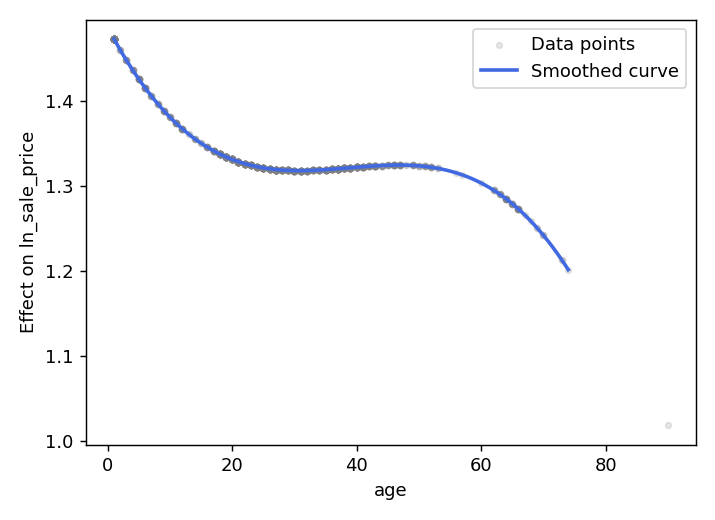
\includegraphics[width=\linewidth]{Figures/orlando_east_age_smooth.png}
    \caption*{\small (a) GAM smooth for age (Orlando East)}
  \end{minipage}
  \hfill
  % right graphic ---------------------------------------------------
  \begin{minipage}[t]{0.48\textwidth}
    \centering
    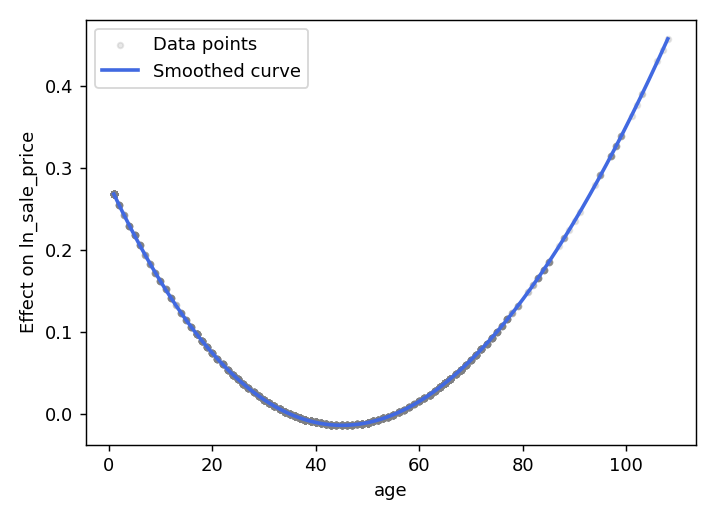
\includegraphics[width=\linewidth]{Figures/orlando_central_age_smooth.png}
    \caption*{\small(b) GAM smooth for age (Orlando Central)}
  \end{minipage}
\end{figure}


\begin{figure}[H]
  \centering
  \begin{minipage}[t]{0.48\textwidth}
    \centering
    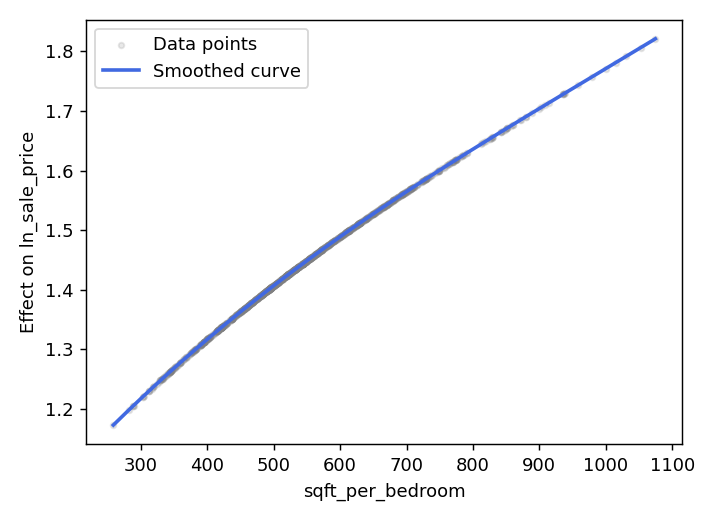
\includegraphics[width=\linewidth]{Figures/orlando_east_sqft_per_bedroom_smooth.png}
    \caption*{\small \centering (c) GAM smooth for sqft per bedroom \par (Orlando East)}
  \end{minipage}
  \hfill
  \begin{minipage}[t]{0.48\textwidth}
    \centering
    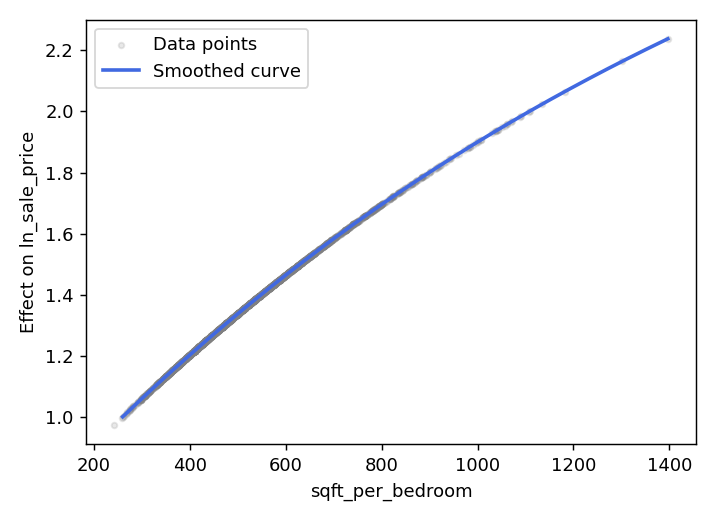
\includegraphics[width=\linewidth]{Figures/orlando_central_sqft_per_bedroom_smooth.png}
    \caption*{\small \centering (d) GAM smooth for sqft per bedroom \par (Orlando Central)}
  \end{minipage}
\end{figure}



\begin{figure}[H]
  \centering
  % left graphic ----------------------------------------------------
  \begin{minipage}[t]{0.48\textwidth}
    \centering
    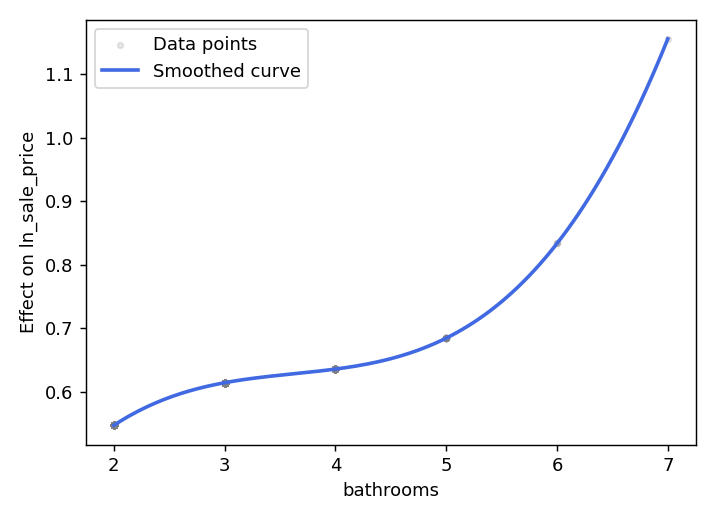
\includegraphics[width=\linewidth]{Figures/orlando_east_bathrooms_smooth.png}
    \caption*{\small(e) GAM smooth for bathrooms (Orlando East)}
  \end{minipage}
  \hfill
  % right graphic ---------------------------------------------------
  \begin{minipage}[t]{0.48\textwidth}
    \centering
    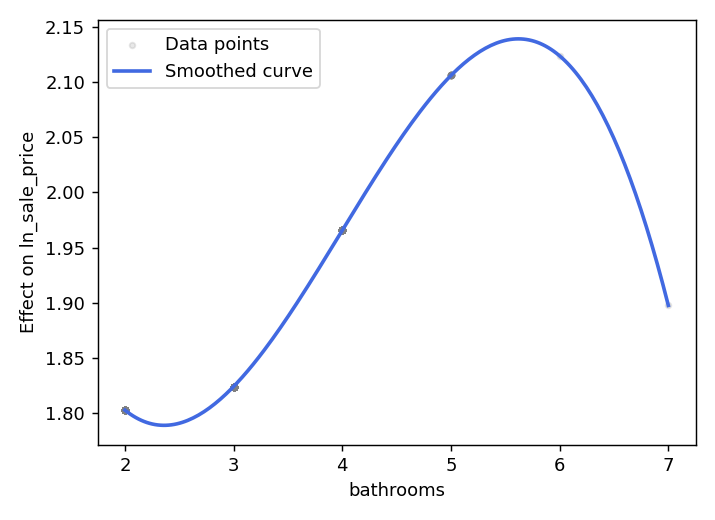
\includegraphics[width=\linewidth]{Figures/orlando_central_bathrooms_smooth.png}
    \caption*{\small(f) GAM smooth for bathrooms (Orlando Central)}
  \end{minipage}
\end{figure}

\begin{figure}[H]
  \centering
  \begin{minipage}[t]{0.48\textwidth}
    \centering
    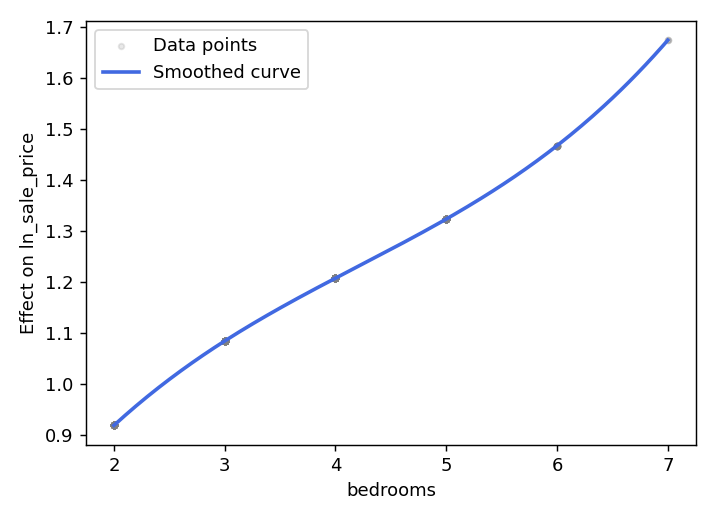
\includegraphics[width=\linewidth]{Figures/orlando_east_bedrooms_smooth.png}
    \caption*{\small(g) GAM smooth for bedrooms (Orlando East)}
  \end{minipage}
  \hfill
  \begin{minipage}[t]{0.48\textwidth}
    \centering
    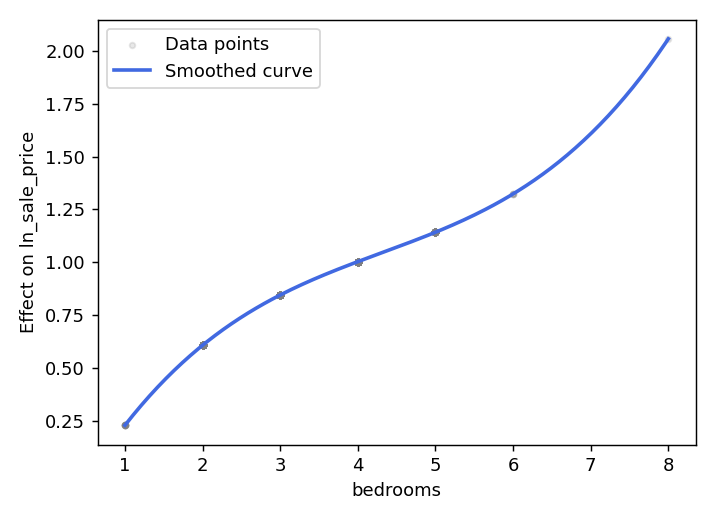
\includegraphics[width=\linewidth]{Figures/orlando_central_bedrooms_smooth.png}
    \caption*{\small (h) GAM smooth for bedrooms (Orlando Central)}
  \end{minipage}
\end{figure}


\begin{figure}[H]
  \centering
  \begin{minipage}[t]{0.48\textwidth}
    \centering
    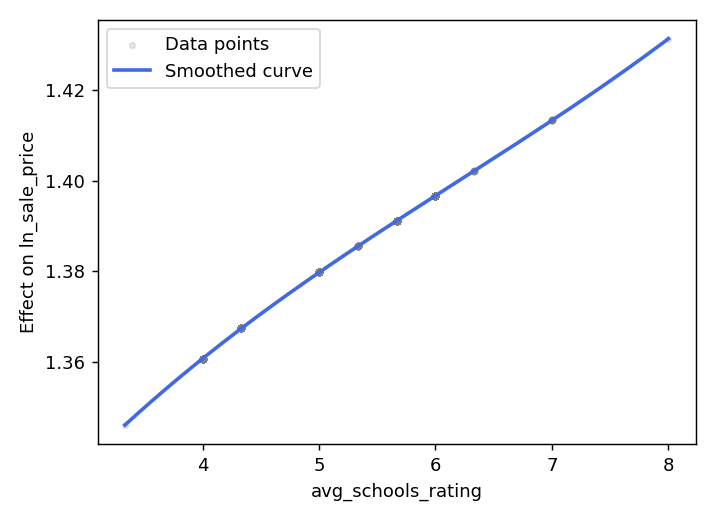
\includegraphics[width=\linewidth]{Figures/orlando_east_avg_schools_rating_smooth.png}
    \caption*{\small \centering (i) GAM smooth for school rating \par (Orlando East)}
  \end{minipage}
  \hfill
  \begin{minipage}[t]{0.48\textwidth}
    \centering
    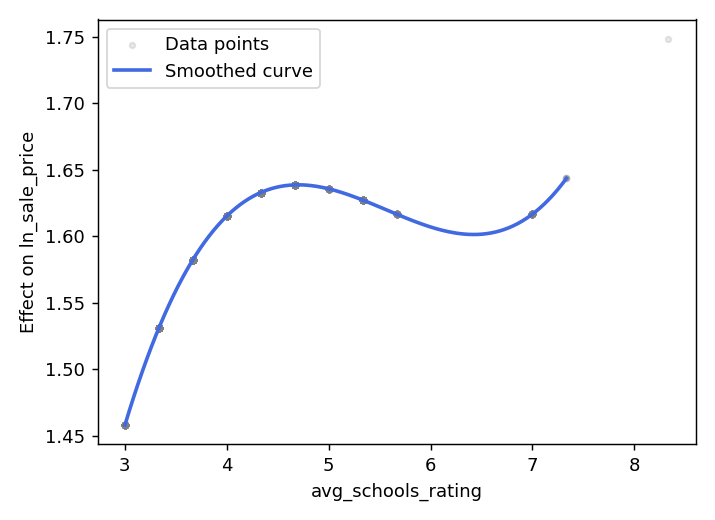
\includegraphics[width=\linewidth]{Figures/orlando_central_avg_schools_rating_smooth.png}
    \caption*{\small \centering (j) GAM smooth for school rating \par (Orlando Central)}
  \end{minipage}
\end{figure}


\begin{figure}[H]
  \centering
  \begin{minipage}[t]{0.48\textwidth}
    \centering
    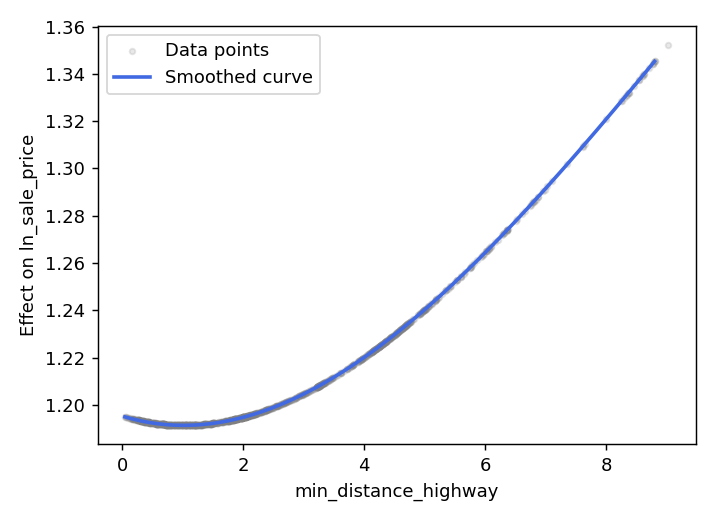
\includegraphics[width=\linewidth]{Figures/orlando_east_min_distance_highway_smooth.png}
    \caption*{\small \centering (k) GAM smooth for min distance to highway \par(Orlando East)}
  \end{minipage}
  \hfill
  \begin{minipage}[t]{0.48\textwidth}
    \centering
    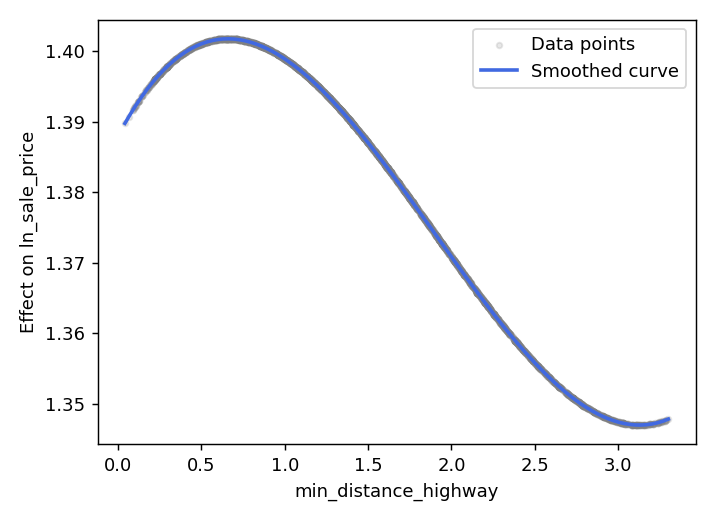
\includegraphics[width=\linewidth]{Figures/orlando_central_min_distance_highway_smooth.png}
    \caption*{\small \centering (l) GAM smooth for min distance to highway \par(Orlando Central)}
  \end{minipage}
\end{figure}


\clearpage


\singlespacing
\nocite{*}
\bibliographystyle{chicago}
\bibliography{../References/PBaikova-References}
\end{document}
